%%!TEX encoding = UTF-8 Unicode

% Several lines in file have comments suggesting common packages for the
% typical thesis in informatics or electronics developed at UA
% uncomment/comment the lines as required for your work
% Before each optional line you will have a small comment

% According to UA rules, font size should range from 10 to 12pt.
\documentclass[11pt,a4paper,openright,twoside,onecolumn]{memoir}

\listfiles
\fixpdflayout

\usepackage[utf8]{inputenc}

% Select Computer Modern Typewritter (For bold ttfamily in listings)
\usepackage{lmodern}
% OR... Bera Mono
%\usepackage[scaled]{beramono} % TTT Font
%\usepackage{anyfontsize} % As the name says...

\usepackage[T1]{fontenc}

% Enable for for Overleaf support
\usepackage{ifthen}
\def\useoverleaf{1}  % change to non-zero (for instance, 1) to enable it

\makeatletter
\newcommand{\makecoverfile}[0]{%
  \immediate\write18{latexmk -pdf cover.tex}%
}
\makeatother

% For PDF merging
\usepackage{pdfpages}

% Set DPI to 300
\pdfpxdimen=\dimexpr 1in/300\relax

% Allow the use of a larger number of packages
\usepackage{morewrites} 

% For English and Portuguese languages
% Portuguese will be the default.
% Uncomment \setlanguage below to change it
\usepackage[english]{babel}

% Uncomment to use a custom date format
%\usepackage{datetime}
%\newdateformat{thesisdate}{\monthname[\THEMONTH] \THEYEAR} % Month Year

% Make pdf look better
\usepackage{microtype} 

% Uncomment to enable floats on facing pages
%\usepackage{dpfloat}

% Side by side figures
% Eg. Fig 1a, Fig 1b
\usepackage[hang,small,bf]{caption}
%\let\tion\undefined
%\let\subfloat\undefined
\usepackage{subcaption}

%\RequirePackage{textcase}

% Dropped Caps
%\usepackage{lettrine}

% Configure Hyperlink color
% As a matter or style, you may use this to enable/disable color boxes on links
%\usepackage[breaklinks=true,colorlinks=false,linkcolor=blue]{hyperref}
% Or use the default values provided by the hyperref package
\usepackage{hyperref}

% Redefine section names according to your preference
%\def\sectionautorefname{Section}
%\def\chapterautorefname{Chapter}
%\def\figureautorefname{Figure}
%\def\listingautorefname{Listing}
%\def\tableautorefname{Table}

% Redefine code boxes
\ifthenelse{\equal{\useoverleaf}{0}}
{\usepackage[outputdir=build]{minted}}
{\usepackage{minted}}%

\addto\captionsportuguese{%
  \renewcommand\listingscaption{Código}
}
\fvset{fontsize=\footnotesize} % Make Code blocks smaller than text
\usepackage{csquotes}

% Add support for PDF Comments
\usepackage{comment}
\ifthenelse{\equal{\useoverleaf}{0}}
{\usepackage{pdfcomment}}{}
\usepackage{bookmark} % New Bookmarks

% For Multiple columns in Glossary
\usepackage{multicol}

% Add support for Math symbols
\usepackage{amsmath}
\usepackage{amssymb}

% Add support for graphics
\usepackage{graphicx}

% Add support for Colors
\usepackage{xcolor}

% Add support for the Euro symbol
\usepackage{eurosym}

% Add support for missingfigure and todo
\usepackage{todonotes}

% Setup bibliography with Biber using IEEE style for proper UTF-8 support
\usepackage[backend=biber, style=ieee, sorting=none, natbib=true, mincitenames=1, maxcitenames=2]{biblatex}
\bibliography{bib/references.bib, bib/rfc.bib}

% Use acronyms
\usepackage[printonlyused]{acronym} % For acronyms

% Indenting the first paragraph after section start
\usepackage{indentfirst}

% For fixing listoflistings with memoir
\usepackage{xparse}

% Uncomment the next lines to enable chart support through pgf and tikz
% This may require you to install further packages in your Tex system
%\usepackage[version=0.96]{pgf}
%\usepackage{tikz}

% UML support
%\usepackage{pgf-umlsd}

% Trees, Arrows, Mindmaps and other popular objects
%\usetikzlibrary{arrows,shadows,trees,shapes,decorations,automata,backgrounds,petri,mindmap} % for pgf-umlsd

% Package to master SI units
\usepackage[detect-weight=true, binary-units=true]{siunitx}
% For Electric Circuits
%\sisetup{load-configurations = binary}

% Set Voltage direction accordingly
% Option : oldvoltagedirection,nooldvoltagedirection,RPvoltages,EFvoltages
% More information at: https://mirrors.ibiblio.org/CTAN/graphics/pgf/contrib/circuitikz/doc/circuitikzmanual.pdf
% By default this template is using the Old Voltage Direction
%\usepackage[oldvoltagedirection,american,cuteinductors,smartlabels]{circuitikz}
%\usetikzlibrary{calc}
%\ctikzset{bipoles/thickness=1}
%\ctikzset{bipoles/length=0.8cm}
%\ctikzset{bipoles/diode/height=.375}
%\ctikzset{bipoles/diode/width=.3}
%\ctikzset{tripoles/thyristor/height=.8}
%\ctikzset{tripoles/thyristor/width=1}
%\ctikzset{bipoles/vsourceam/height/.initial=.7}
%\ctikzset{bipoles/vsourceam/width/.initial=.7}
%\tikzstyle{every node}=[font=\small]
%\tikzstyle{every path}=[line width=0.8pt,line cap=round,line join=round]

% For inline TT text (e.g. code snippets)
\usepackage{verbatim}

% Frames around figures and allow force placement
\usepackage{float}

% Configure Float style
%\floatstyle{boxed}
%\restylefloat{table}
%\restylefloat{figure}
%\restylefloat{lstlisting}

% For test purposes you may use the lipsum package to create dummy text
\usepackage{lipsum} % REMOVE

%Keep floats inside section!
\usepackage[section]{placeins}
\let \oldsubsubsection \subsubsection
\renewcommand{\subsubsection}[2][]{
  \FloatBarrier
  \oldsubsubsection#1{#2}
}
\let \oldsubsection \subsection
\renewcommand{\subsection}[2][]{
  \FloatBarrier
  \oldsubsection#1{#2}
}
\let \oldsection \section
\renewcommand{\section}[2][]{
  \FloatBarrier
  \oldsection#1{#2}
}
\let \oldchapter \chapter
\renewcommand{\chapter}[2][]{
  \FloatBarrier
  \oldchapter#1{#2}
}



% Use the built-in division styling
\headstyles{memman}

% Include subsections in the TOC
\settocdepth{subsection}

% Numbering down to subsections as well
\setsecnumdepth{subsection}

% extra index for first lines
\makeindex[lines]

% Margins for University of Aveiro Thesis
\setlrmarginsandblock{3cm}{2.5cm}{*}
\setulmarginsandblock{3cm}{3cm}{*}
\checkandfixthelayout

% Or select your custom spacing to make any ajustment
%\addtolength{\parskip}{0.5\baselineskip}
\linespread{1.5}

\newcommand\mainmatterWithoutReset
{\edef\temppagenumber{\arabic{page}}%
  \mainmatter
  \setcounter{page}{\temppagenumber}%
}


%%%%%%%%%%%%%%%%%%%%%%%%%%%%%%%%%%%%%%%%%%%%%%%%%%
% Document begins here
%%%%%%%%%%%%%%%%%%%%%%%%%%%%%%%%%%%%%%%%%%%%%%%%%%

\begin{document}
\ifthenelse{\equal{\useoverleaf}{0}}{}{\makecoverfile{}}%

\includepdf[pages=-]{cover.pdf}

% Uncomment to enable English
%\selectlanguage{english}


% Front matter

%Custom Chapter style named `thesis`
\makechapterstyle{thesis}{% Based on ell
  \chapterstyle{default}
  \renewcommand*{\chapnumfont}{\normalfont\sffamily}
  \renewcommand*{\chaptitlefont}{\normalfont\Huge\sffamily}
  \settowidth{\chapindent}{\chapnumfont 111}
  \renewcommand*{\chapterheadstart}{\begingroup
    \vspace*{\beforechapskip}%
    \begin{adjustwidth}{}{-\chapindent}%
    \hrulefill
    \smash{\rule{0.4pt}{15mm}}
    \end{adjustwidth}\endgroup}
  \renewcommand*{\printchaptername}{}
  \renewcommand*{\chapternamenum}{}
  \renewcommand*{\printchapternum}{%
    \begin{adjustwidth}{}{-\chapindent}
    \hfill
    \raisebox{10mm}[0pt][0pt]{\fontsize{30}{25}\selectfont\chapnumfont \thechapter}%
                              \hspace*{1em}
    \end{adjustwidth}\vspace*{-3.0\onelineskip}}
  \renewcommand*{\printchaptertitle}[1]{%
    \vskip\onelineskip
    \raggedleft {\chaptitlefont ##1}\par\nobreak\vskip 4\onelineskip}}


% Select chapter style from existing or select custom
%\chapterstyle{thesis} % Others: dowding, demo2, dash, chappell, brotherton, bianchi, ger, madsen, tatcher, veelo,indexes)
% thesis can also be used as defined previously
% Check the memoir documentation for the available themes
% Default is veelo
\chapterstyle{veelo}
\makeoddfoot{plain}{}{\thepage}{} % Added by André Zúquete to fix a page numbering issue on the veelo chapter style


% If you feel adventurous you can also define all aspects of your theme
% Use either this input or the chapterstyle before
% \input{custom-theme.tex}

%Exclude sub figures from List of Figures
%\captionsetup[subfloat]{list=no}

% Texts
\newenvironment{introduction}
{%
  \begin{minipage}{\textwidth}%
   \itshape%
}
{%
  \end{minipage}%
  \par\addvspace{2\baselineskip plus 0.2\baselineskip minus 0.2\baselineskip}%
}

% Select Page style
\pagestyle{plain}


\frontmatter

\tightlists
\midsloppy
\raggedbottom

\setcounter{tocdepth}{2} %subsections are added to the TOC
\setcounter{secnumdepth}{4} %subsubsections are numbered

% Initial document tables start here: TOC, LOF, LOT, Glossary
% Table of contents with slightly smaller font
\cleardoublepage
{\small\tableofcontents}

% List of figures with slightly smaller font
\cleardoublepage
{\small\listoffigures}

% List of tables with slightly smaller font
\cleardoublepage
{\small\listoftables}

% List of code snippets

% Fix for Listings with memoir

\RenewDocumentCommand \chapter { s O{#3} m }{%
  \FloatBarrier
  \IfValueTF{#1}  % if optional star is seen
    {\oldchapter*{#2}}
    {\oldchapter#1{#2}}
}

\renewcommand{\listingscaption}{Código}
\renewcommand{\listoflistingscaption}{Lista de Excertos de Código}
\cleardoublepage
{\small\listoflistings}
\addcontentsline{toc}{chapter}{\listoflistingscaption}

% Reset Chapters
\renewcommand{\chapter}[2][]{
  \FloatBarrier
  \oldchapter#1{#2}
}

% Print Glossary
{\small\chapter{Glossário}

\footnotesize
\SingleSpacing

\begin{multicols}{2}
\begin{acronym}[AAAAAA]

	\acro{h2o}[H2O]{Water}
	\acro{adsl}[ADSL]{Asymmetric Digital Subscriber Line}
	\acro{cctv}[CCTV]{Closed Circuit Television}
	\acro{ai}[AI]{Artificial Intelligence}
	\acro{iou}[IoU]{Intersection over Union}
	\acro{bb}[BB]{Bounding Box}
	\acro{us}[US]{United States}
	\acro{ap}[AP]{Average Precision}
	\acro{map}[mAP]{Mean Average Precision}
	\acro{yolo}[YOLO]{You Only Look Once}
	\acro{ssd}[SSD]{Single Shot Detection}
	\acro{frcnn}[Faster-RCNN]{Faster Region-based Convolutional Neural Networks}
	\acro{dcnns}[DCNNs]{Deep Convolutional Neural Network}
	\acro{cnn}[CNN]{Convolutional Neural Network}
	\acro{rcnn}[R-CNN]{Region-based Convolutional Neural Network}
	\acro{dl}[DL]{Deep Learning}
	\acro{gpu}[GPU]{Graphical Processing Unit}
	\acro{cpu}[CPU]{Central Processing Unit}
	\acro{tpu}[TPU]{Tensor Processing Unit}
	\acro{cuda}[CUDA]{Compute Unified Device Architecture}
	\acro{e2e}[E2E]{End-to-End}
\end{acronym}
\end{multicols}

}

%%%%%%%%%%%%%%%%%%%%%%%%%%%%%%%%%%%%%%%%%%%%%%%%%%%%%%%
% Main document starts here
%%%%%%%%%%%%%%%%%%%%%%%%%%%%%%%%%%%%%%%%%%%%%%%%%%%%%%%

\mainmatter

% Line spacing: 1.5 pt 
\OnehalfSpacing

%%%%%%%%%%%%%%%%%%%%%%%%%%%%%%%%%%%%%%%%%%%%%%%%%%%%%%%
% Start of Thesis text 
%%%%%%%%%%%%%%%%%%%%%%%%%%%%%%%%%%%%%%%%%%%%%%%%%%%%%%%

% Uncomment to add further chapters
\chapter{Introduction}
\label{chapter:introduction}

\newenvironment{introduction2}
{\quote\itshape}
{\endquote}

\begin{introduction2}
\end{introduction2}

\section{Context and Motivation}
In recent years, there has been an alarming increase in firearm-related crime. In 2022, the Federal Bureau of 
Investigation reported fifty active shooter incidents in the \ac{us}. These were spread across 25 states, 
and 313 casualties in these incidents, 
Figure \ref{fig:casualties}, including 100 deaths and 213 injuries, with the most severe incident causing seven 
fatalities and 48 injuries \selectlanguage{english}\cite{rfc37}.

Notably, there was a 18\% decrease in such incidents in 2021 but a significant 66.7\% increase compared to 2018, as shown in Figure \ref{fig:incidents}.

\begin{figure}[h]
    \centering
    \begin{minipage}{0.42\textwidth}
        \centering
        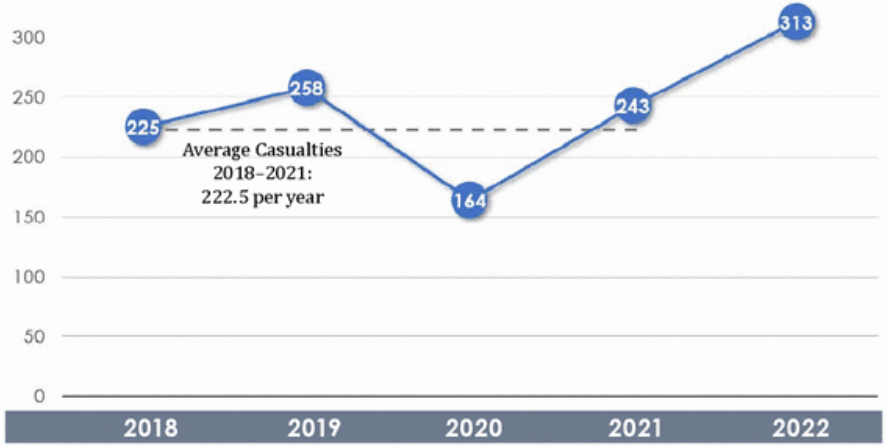
\includegraphics[width=1\linewidth]{figs/active-shooter-incidents.png}
        \caption{Active shooter incidents casualties in the \ac{us} \selectlanguage{english}\cite{rfc37}}
        \label{fig:casualties}
    \end{minipage}\hfill
    \begin{minipage}{0.45\textwidth}
        \centering
        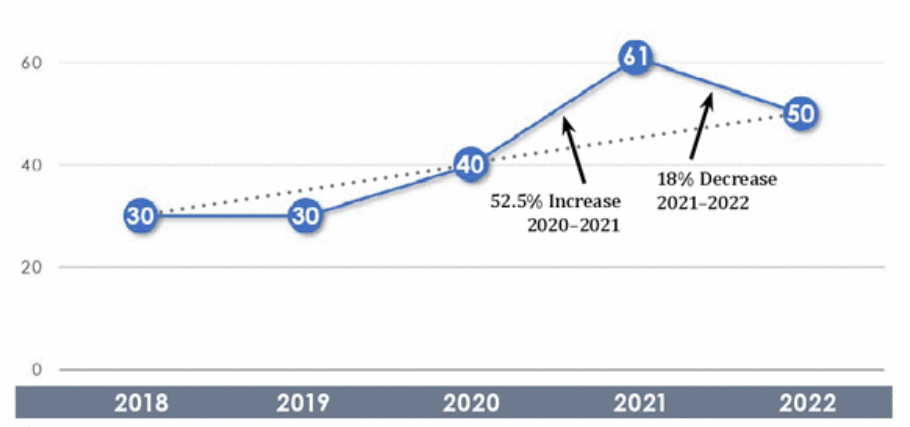
\includegraphics[width=1\linewidth]{figs/active-shooter-us.png}
        \caption{Active shooter incidents in the \ac{us} \selectlanguage{english}\cite{rfc37}}
        \label{fig:incidents}
    \end{minipage}
\end{figure}

Despite the existence of strict gun laws in numerous countries, the accessibility of firearms remains relatively 
high. The \ac{us} is the global leader in civilian gun ownership, with an estimated 120.5 firearms per 100 
people, which is nearly twice as high as the country with the second-highest rate.

Despite the existence of strict gun laws in many countries, firearm access remains relatively 
easy \selectlanguage{english}\cite{rfc39, rfc40}. The \ac{us} is the global leader in civilian gun 
ownership, with an estimated 120.5 firearms per 100 
people, which is nearly twice as high as the country with the second-highest rate.
\selectlanguage{english}\cite{rfc32}.

Within the 50 active shooter incidents in 2022, a total of 61 firearms were utilized, as shown in Figure \ref{fig:fbi-firearms}. Handguns were the most frequently used, accounting for 29 of the weapons, followed closely by rifles at 26.

\begin{figure}[h]
    \centering 
    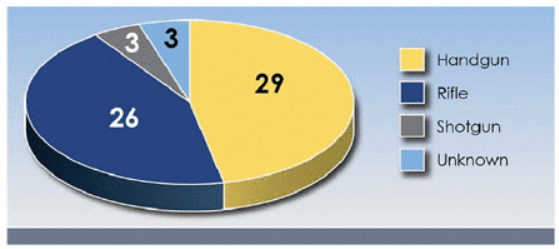
\includegraphics[width=0.4\textwidth]{figs/firearms.png} 
    \caption{Firearm used by active shooters in the \ac{us} \selectlanguage{english}\cite{rfc37}}
    \label{fig:fbi-firearms}
\end{figure}

In relation to Portugal, as RASI  \selectlanguage{english}\cite{rfc41}, reports, there has been a substantial 
increase in criminal activity. The total number of general crime reports registered 
by the Public Security Forces was 343845 in 2022, which is an increase of 42451 compared to 2021, 
representing a 14.1\% rise. Specifically, the total number of reported violent and serious crimes was 
13281, up by 1667 from the previous year, marking a 14.4\% increase, as shown in Figure \ref{fig:crimes-portugal}.

\begin{figure}[h]
    \centering 
    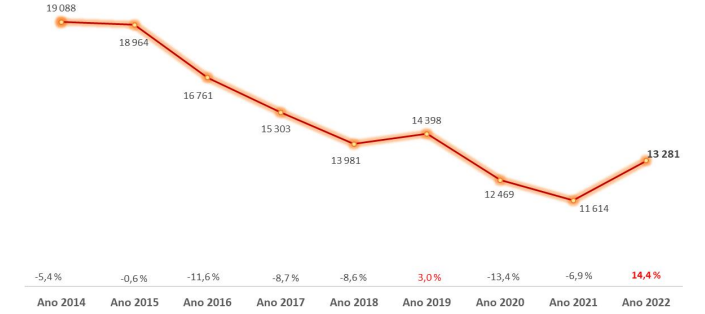
\includegraphics[width=0.8\textwidth]{figs/crimes-portugal.png} 
    \caption{Crime Rates in Portugal from 2014 to 2022 \selectlanguage{english}\cite{rfc41}}
    \label{fig:crimes-portugal}
\end{figure}

Figure \ref{fig:geo-crimes} shows a geographically decrease in the districts of Braga (-5.1\%), Bragança (-17.9\%), and Vila Real (-10\%). Conversely, there was a significant increase in Lisbon (+11.4\%), Porto (+11.3\%), Faro (+23.9\%), and the Autonomous Region of Madeira (+52\%).

\begin{figure}[h]
    \centering 
    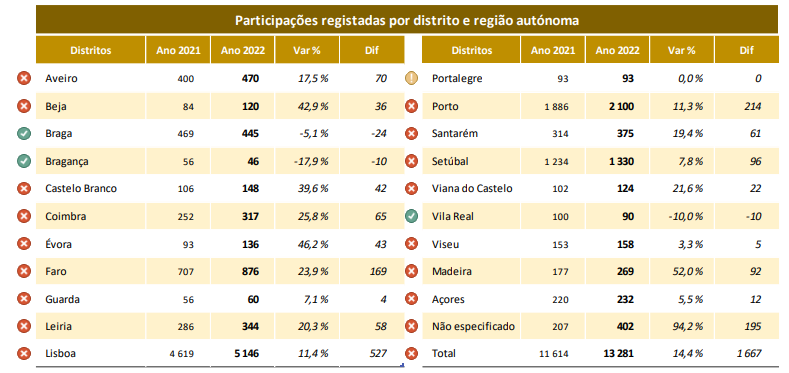
\includegraphics[width=0.7\textwidth]{figs/geo-crimes-rate.png} 
    \caption{Geographical Distribution of Crime Rate Increase in Portugal by District in 2022 \selectlanguage{english}\cite{rfc41}}
    \label{fig:geo-crimes}
\end{figure}

Along the years, It was noticed that \ac{cctv} systems have became a 
crucial tool for crime prevention. Research indicates a 
correlation between \ac{cctv} deployment and a reduction in crime rates, especially in car parks 
\selectlanguage{english}\cite{rfc33}. For example, in Florida, the implementation of \ac{cctv} has resulted in 
crime rate reductions of up to 51\% in certain areas \selectlanguage{english}\cite{rfc34}. Alongside its growing 
popularity worldwide, \ac{cctv} surveillance has generated debates concerning its effectiveness, efficiency, and 
related privacy issues. Critics of \ac{cctv} surveillance frequently raise concerns about the invasion of privacy 
and the risk of violating privacy laws \selectlanguage{english}\cite{rfc38}.

A significant challenge in operating \ac{cctv} systems is the reliance on human monitoring, which is susceptible to errors due to fatigue or distraction. Additionally, the financial implications of \ac{cctv}, including the costs associated with constructing and maintaining these surveillance systems, form an essential part of the discussion. These costs must be weighed against the potential benefits in crime reduction and public safety \selectlanguage{english}\cite{rfc38}. 

The effectiveness of \ac{cctv} in controlling crime varies and is influenced by several factors, including geographic location, crime types, and the strategies employed for camera monitoring. Studies have revealed that \ac{cctv} operations managed by private security personnel tend to have a more substantial crime prevention impact compared to those overseen by police \selectlanguage{english}\cite{rfc36}. In Sweden's deprived neighborhoods, the use of \ac{cctv} has led to a decrease in violent crimes, though it has not significantly affected property crime rates or the clearance of crimes \selectlanguage{english}\cite{rfc35}.

\ac{cctv} systems have emerged as key tools in crime prevention, offering the ability to reduce specific types of crime, especially in environments where they are actively monitored and used alongside other interventions \selectlanguage{english}\cite{rfc35}. 
\section{Objectives}
The primary goal of this project is to advance in the field of public safety and security through the development of a Deep Learning-Based system for real-time weapon detection in \ac{cctv} surveillance footage, designed for the detection and classification of weapons, such as firearms and knives. This includes several key aspects:
\begin{itemize}
    \item Exploration of Current Technologies and Methods: thorough review of the state-of-the-art technologies and methodologies used in real-time, analyzing existing approaches' effectiveness, efficiency, and applicability in various real-world scenarios;
    \item Identification and Analysis of Public Databases: identify public databases that contain relevant data on anomalous objects;
    \item Development of a Deep Learning Model: develop a state-of-the-art deep learning model capable of accurately identifying and classifying firearms or knives in diverse and challenging surveillance scenarios;
    \item Architecture Design and Prototyping: proposing and developing a prototype solution with a well-defined architecture;
    \item Performance Evaluation and Limitation Analysis: extensive testing of the prototype in various real-life scenarios to evaluate its performance, accuracy, and reliability;
\end{itemize}

The expectation is that the application and model developed through this research will surpass existing solutions in terms of efficiency, accuracy, and practicality. To achieve this, it is imperative to conduct a comprehensive analysis of the work done by other researchers. This examination will not only provide insights into the most effective strategies and methodologies but will also shed light on the common challenges and barriers encountered in similar attempts.  
\section{Outline of the Document}
The document is organized into subsequent chapters as follows: 

\begin{itemize}
    \item Chapter 2 offers a detailed analysis of the 
    existing research and technologies in weapon detection, focusing on critical aspects like weapon categorization, 
    the significance of \ac{cctv}, and the application of deep learning algorithms;
    \item Chapter 3 discusses the high-level architecture of the project and details the work plan, including 
    milestones and a Gantt chart to illustrate the project timeline;
    \item Chapter 4 describes the implementation of the application, including the system architecture and a 
    comprehensive examination of each component involved in the development process;
    \item Chapter 5 presents the tests conducted and the results obtained, providing a thorough analysis of 
    the performance and accuracy of the implemented system;
    \item Chapter 6 concludes the thesis by summarizing the key findings, discussing the implications of the 
    results, and suggesting directions for future work in the field of weapon detection.
\end{itemize}

\renewcommand{\arraystretch}{2}
\renewcommand{\figurename}{Figure}
\chapter{Concepts and Related Work}
\label{chapter:literarure}

\newenvironment{literature}
{\quote\itshape}
{\endquote}

\begin{literature}
This chapter presents the concepts/technologies related to the application domain and the related work that could 
be used to inform our options for an approach.
 The discussion begins with an overview of the general context in Section 2.1, laying the 
 groundwork for a more detailed examination of weapon detection technologies and \ac{cctv} systems. Section 2.2 
 delves into object detection, reviewing key algorithms and techniques. Section 2.3 focuses on related research, 
 including methodologies, \ac{cctv} setup, and weapon detection analysis. It concludes with a comprehensive 
 examination of datasets and architectural methods in weapon detection research.
\end{literature}

\section{Domain-related concepts/technologies}
These sections support the background knowledge needed to understand some of the concepts and technologies in use along our work.
\subsection{Weapons}
In order to have a system that detects weapons on video footage, we need an understanding of a basic concept: 
the definition and types of weapons.  Therefore, the Cambridge Dictionary\footnote{https://dictionary.cambridge.org/dictionary/english/weapon  [Accessed on: November,2023]} defines a weapon 
as "any object used in fighting or war, such as a gun, bomb, knife, etc.". This definition implies that a weapon 
is a tool or instrument  that is intended to cause damage or injury, whether to 
living beings, structures or systems. Weapons have a wide range of uses, such as hunting, self-defense or warfare. 
However, their fundamental purpose 
remains unchanged: they amplify the user's ability to exert force, in either an offensive or defensive capacity.

They are categorized based on diferent criteria: range, mechanism and intented use.
However, two categories, firearms and close-combat weapons, will be the main focus of this study.

Melee weapons are close-combat instruments that require the user to be in direct proximity to their target, 
like swords, daggers, maces, and clubs.

Firearms are a subset of ranged weapons that discharge projectiles powered by rapidly expanding high-pressure gas 
from chemical reactions. They can be categorized into:
\begin{itemize}
    \item Handguns: Small, handheld firearms like pistols and revolvers.
    \item Rifles: Designed for accuracy, rifles have a longer barrel and are often used in situations requiring precision.
    \item Shotguns: These fire shells that contain multiple pellets, making them effective at close range.
    \item Automatic and Semi-Automatic: Automatic firearms continuously fire bullets as long as the trigger is pressed, while semi-automatics require a trigger pull for each shot.
\end{itemize}

Figure \ref{fig:first_image} shows an example of a melee weapon, while 
Figure \ref{fig:second_image} presents various types of firearms, showcasing the diversity in firearm design and 
functionality.

\begin{figure}[h]
    \centering
    \begin{minipage}{0.45\textwidth}
        \centering
        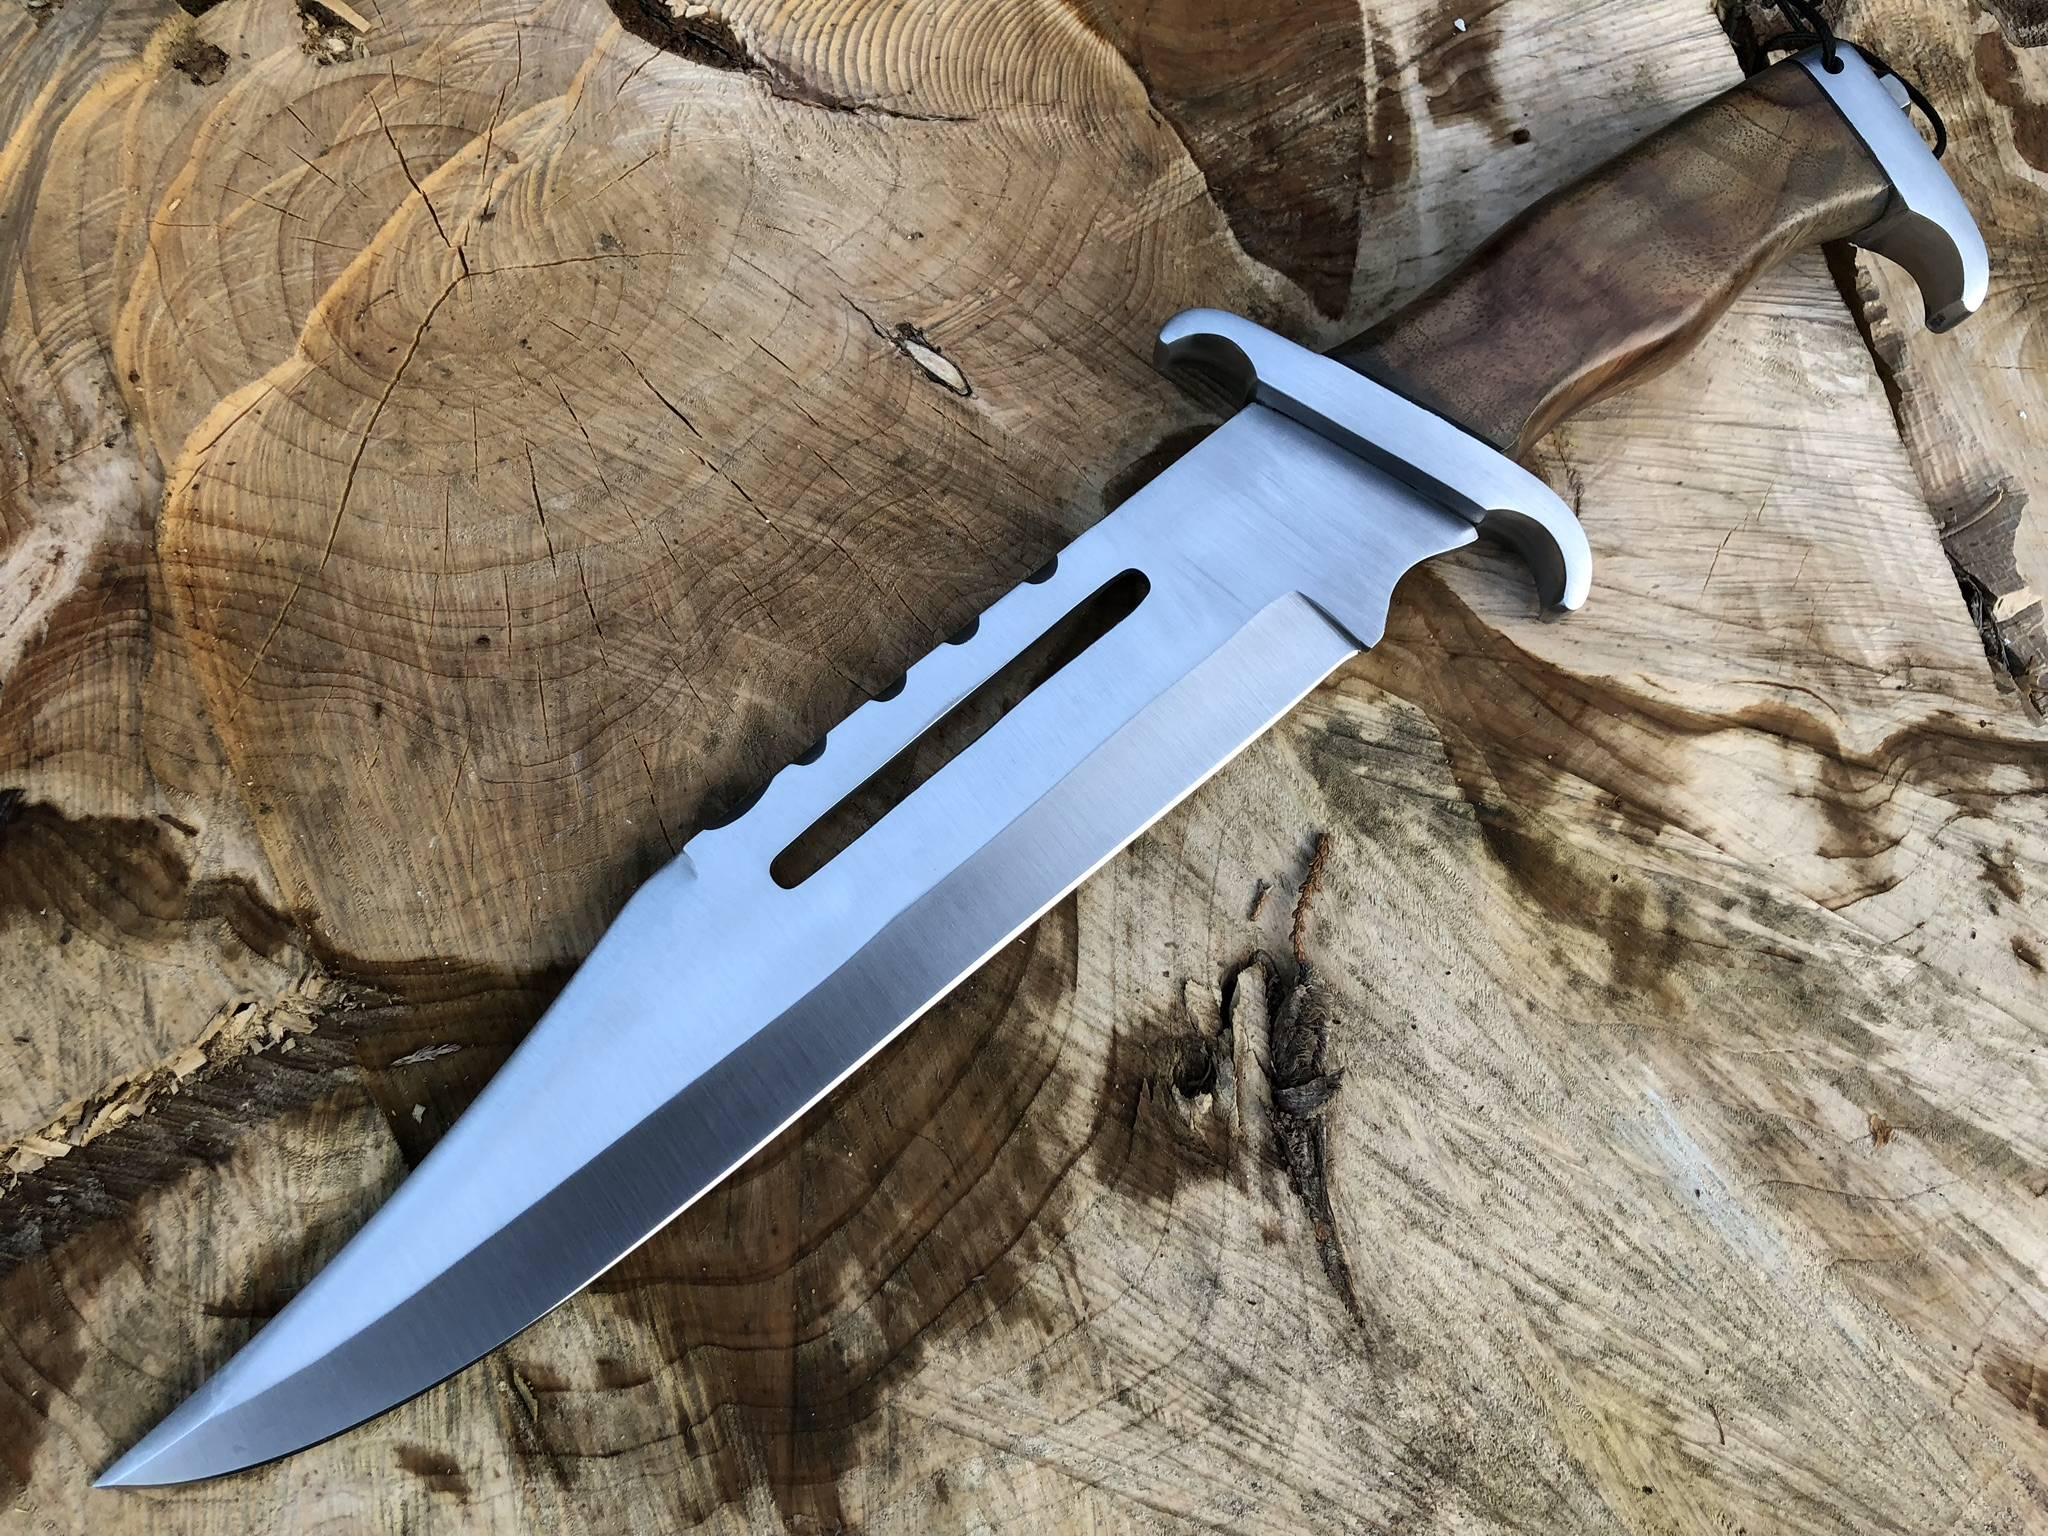
\includegraphics[width=1\linewidth]{figs/knife.jpg}
        \caption{Melee Weapon Example}
        \label{fig:first_image}
    \end{minipage}\hfill
    \begin{minipage}{0.48\textwidth}
        \centering
        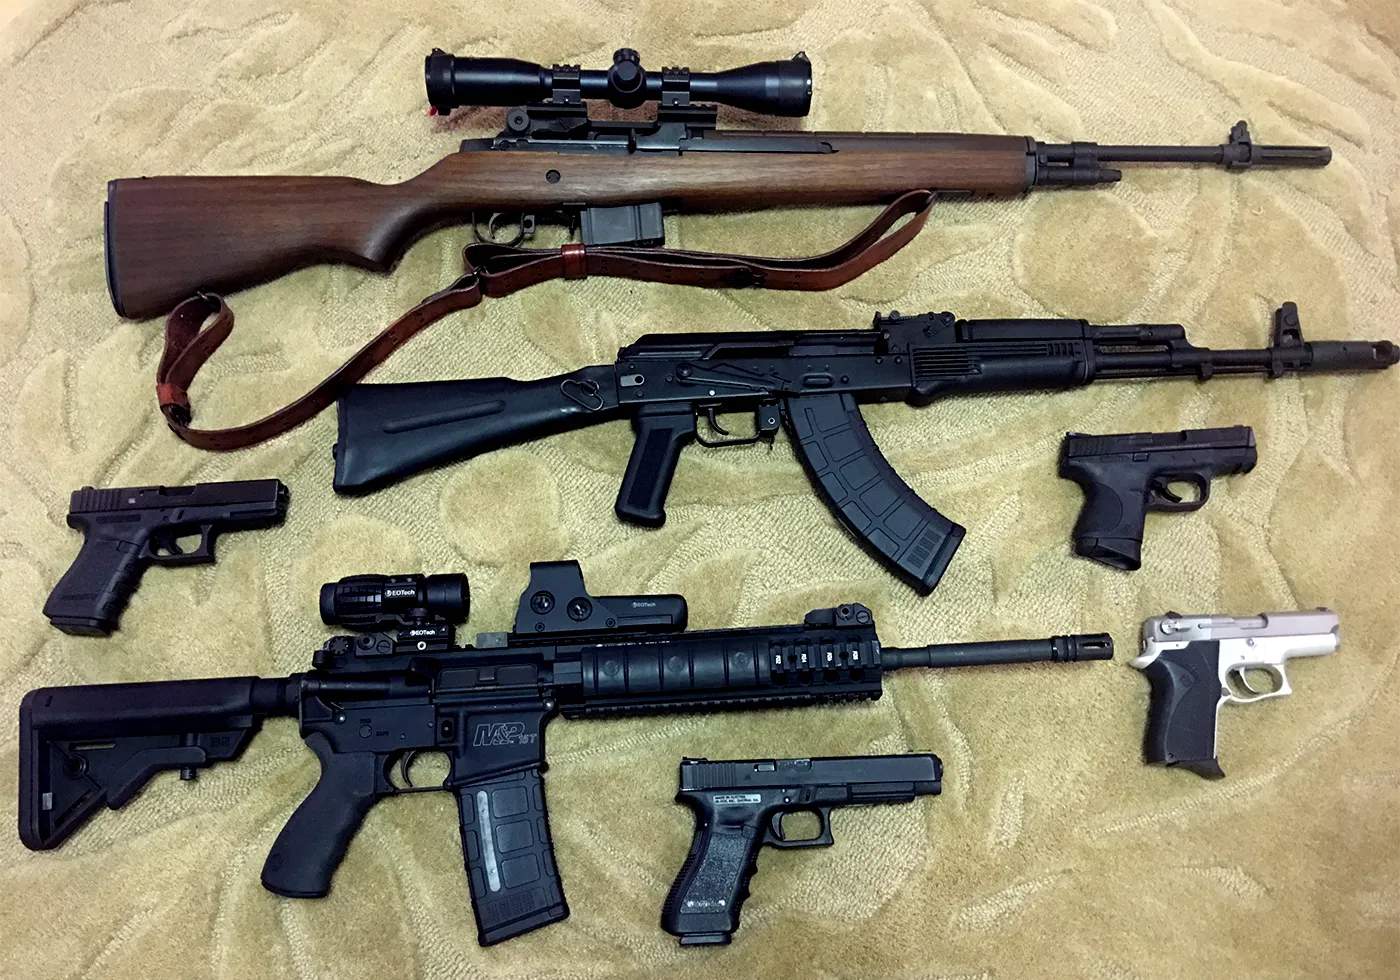
\includegraphics[width=1\linewidth]{figs/firearm.png}
        \caption{Different Firearms Example}
        \label{fig:second_image}
    \end{minipage}
\end{figure}

\subsection{\ac{cctv}}
\ac{cctv} refers to a video surveillance system with strategically positioned cameras in various locations. These cameras capture footage, which is then transmitted to monitors for both real-time observation and later playback.

\begin{figure}[h]
    \centering
    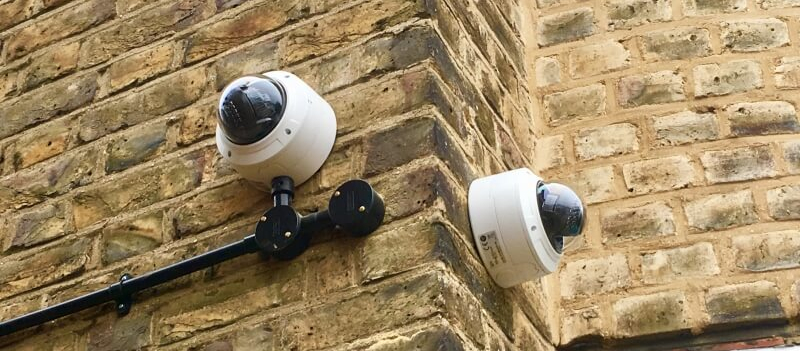
\includegraphics[width=0.42\textwidth]{figs/cctv.jpg}
    \hfill
    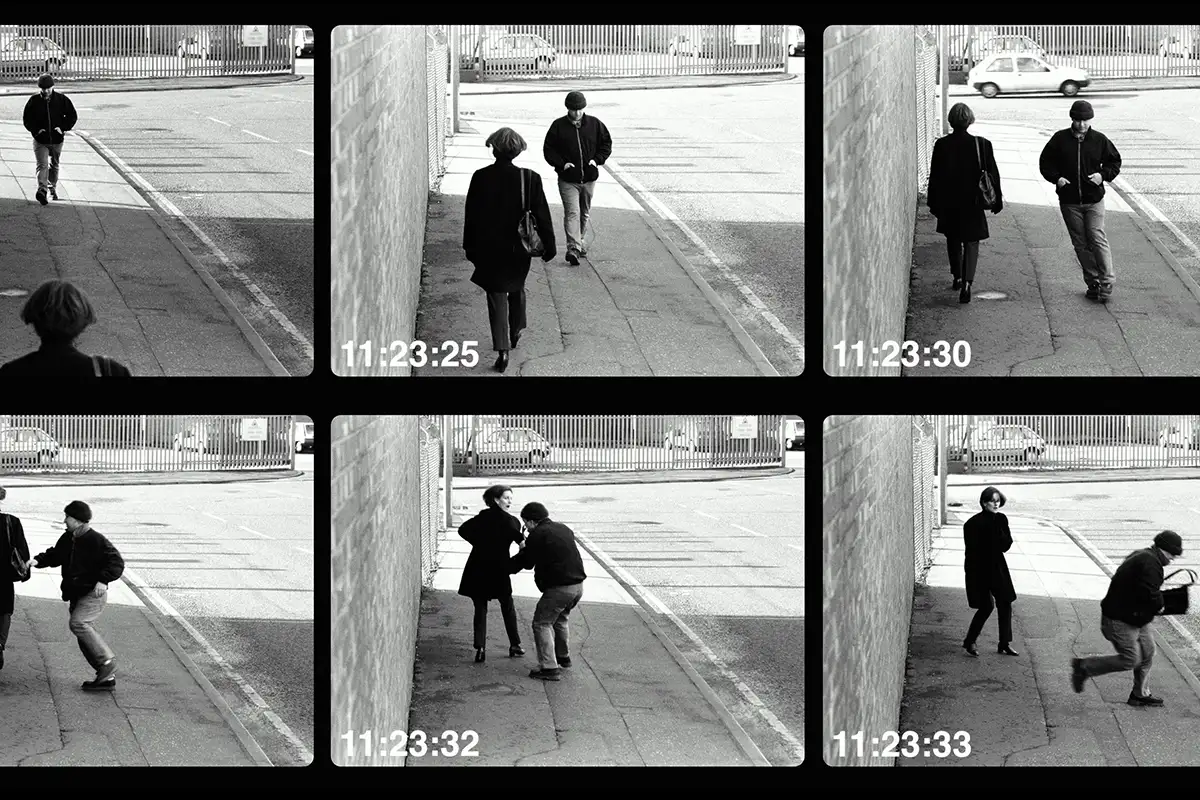
\includegraphics[width=0.42\textwidth]{figs/cctv-footage.png}
    \caption{\ac{cctv} Cameras (Left Image) and \ac{cctv} Footage Samples (Right Image)}
    \label{fig:cctv-and-footage}
\end{figure}

The primary goal of a \ac{cctv} system is to enhance area security through persistent surveillance of key areas. This 
is highly beneficial for large spaces or sites containing valuable or sensitive items. Besides recording, these systems 
can issue alerts for detected motion, especially during off-hours in vacant business premises. These alerts are crucial 
for quickly informing authorities about possible security threats. 

Additionally, surveillance systems are instrumental 
in monitoring activities during both operational and non-operational hours and serve as crucial tools in identifying 
suspects in criminal activities.

\subsection{\ac{cctv} Setup and Configuration}
Ensuring the effectiveness of a \ac{cctv} security system requires careful consideration of several key factors.
\begin{itemize}
    \item Environmental Context Analysis:
        \begin{itemize}
            \item Understand the specific crime dynamics of the area;
            \item Strategically position cameras to cover high-risk zones;
        \end{itemize}
    \item Line-of-Sight Optimization:
    \begin{itemize}
        \item Ensure clear visibility for each camera;
        \item Minimize obstructions such as immovable objects and foliage;
    \end{itemize}
    \item Regular Maintenance:
    \begin{itemize}
        \item Clear any new obstructions that may arise;
        \item Perform routine checks and updates to maintain system functionality.
    \end{itemize}
\end{itemize}

The design of the cameras significantly influences their ability to prevent crime. Semi-covert 'dome' 
cameras, like the camera showed in figure \ref{fig:semi-dome}, are often more effective in discouraging criminal activities compared 
to overt cameras, figure \ref{fig:covert}, making them an ideal option in many scenarios. An effective 
\ac{cctv} system is not just about installation but also involves active monitoring and prompt enforcement 
actions \selectlanguage{english}\cite{rfc4}.
\begin{figure}[h]
    \centering

    % Image 1
    \begin{minipage}{0.3\textwidth}
        \centering
        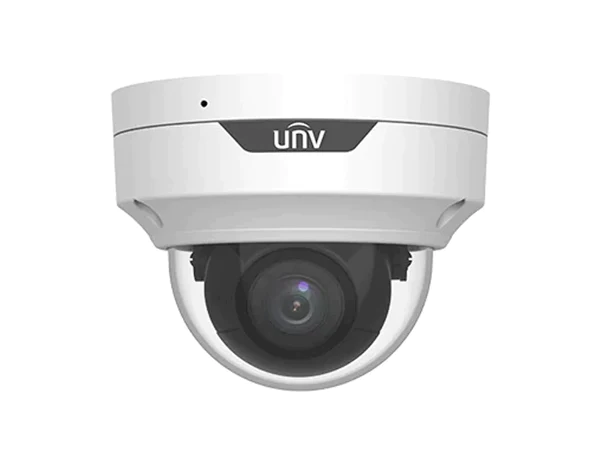
\includegraphics[width=\textwidth]{figs/semi-dome.png} % Include the image
        \caption{Semi-covert dome camera}
        \label{fig:semi-dome}
    \end{minipage}
    \hspace{2cm}
    % Image 2
    \begin{minipage}{0.32\textwidth}
        \centering
        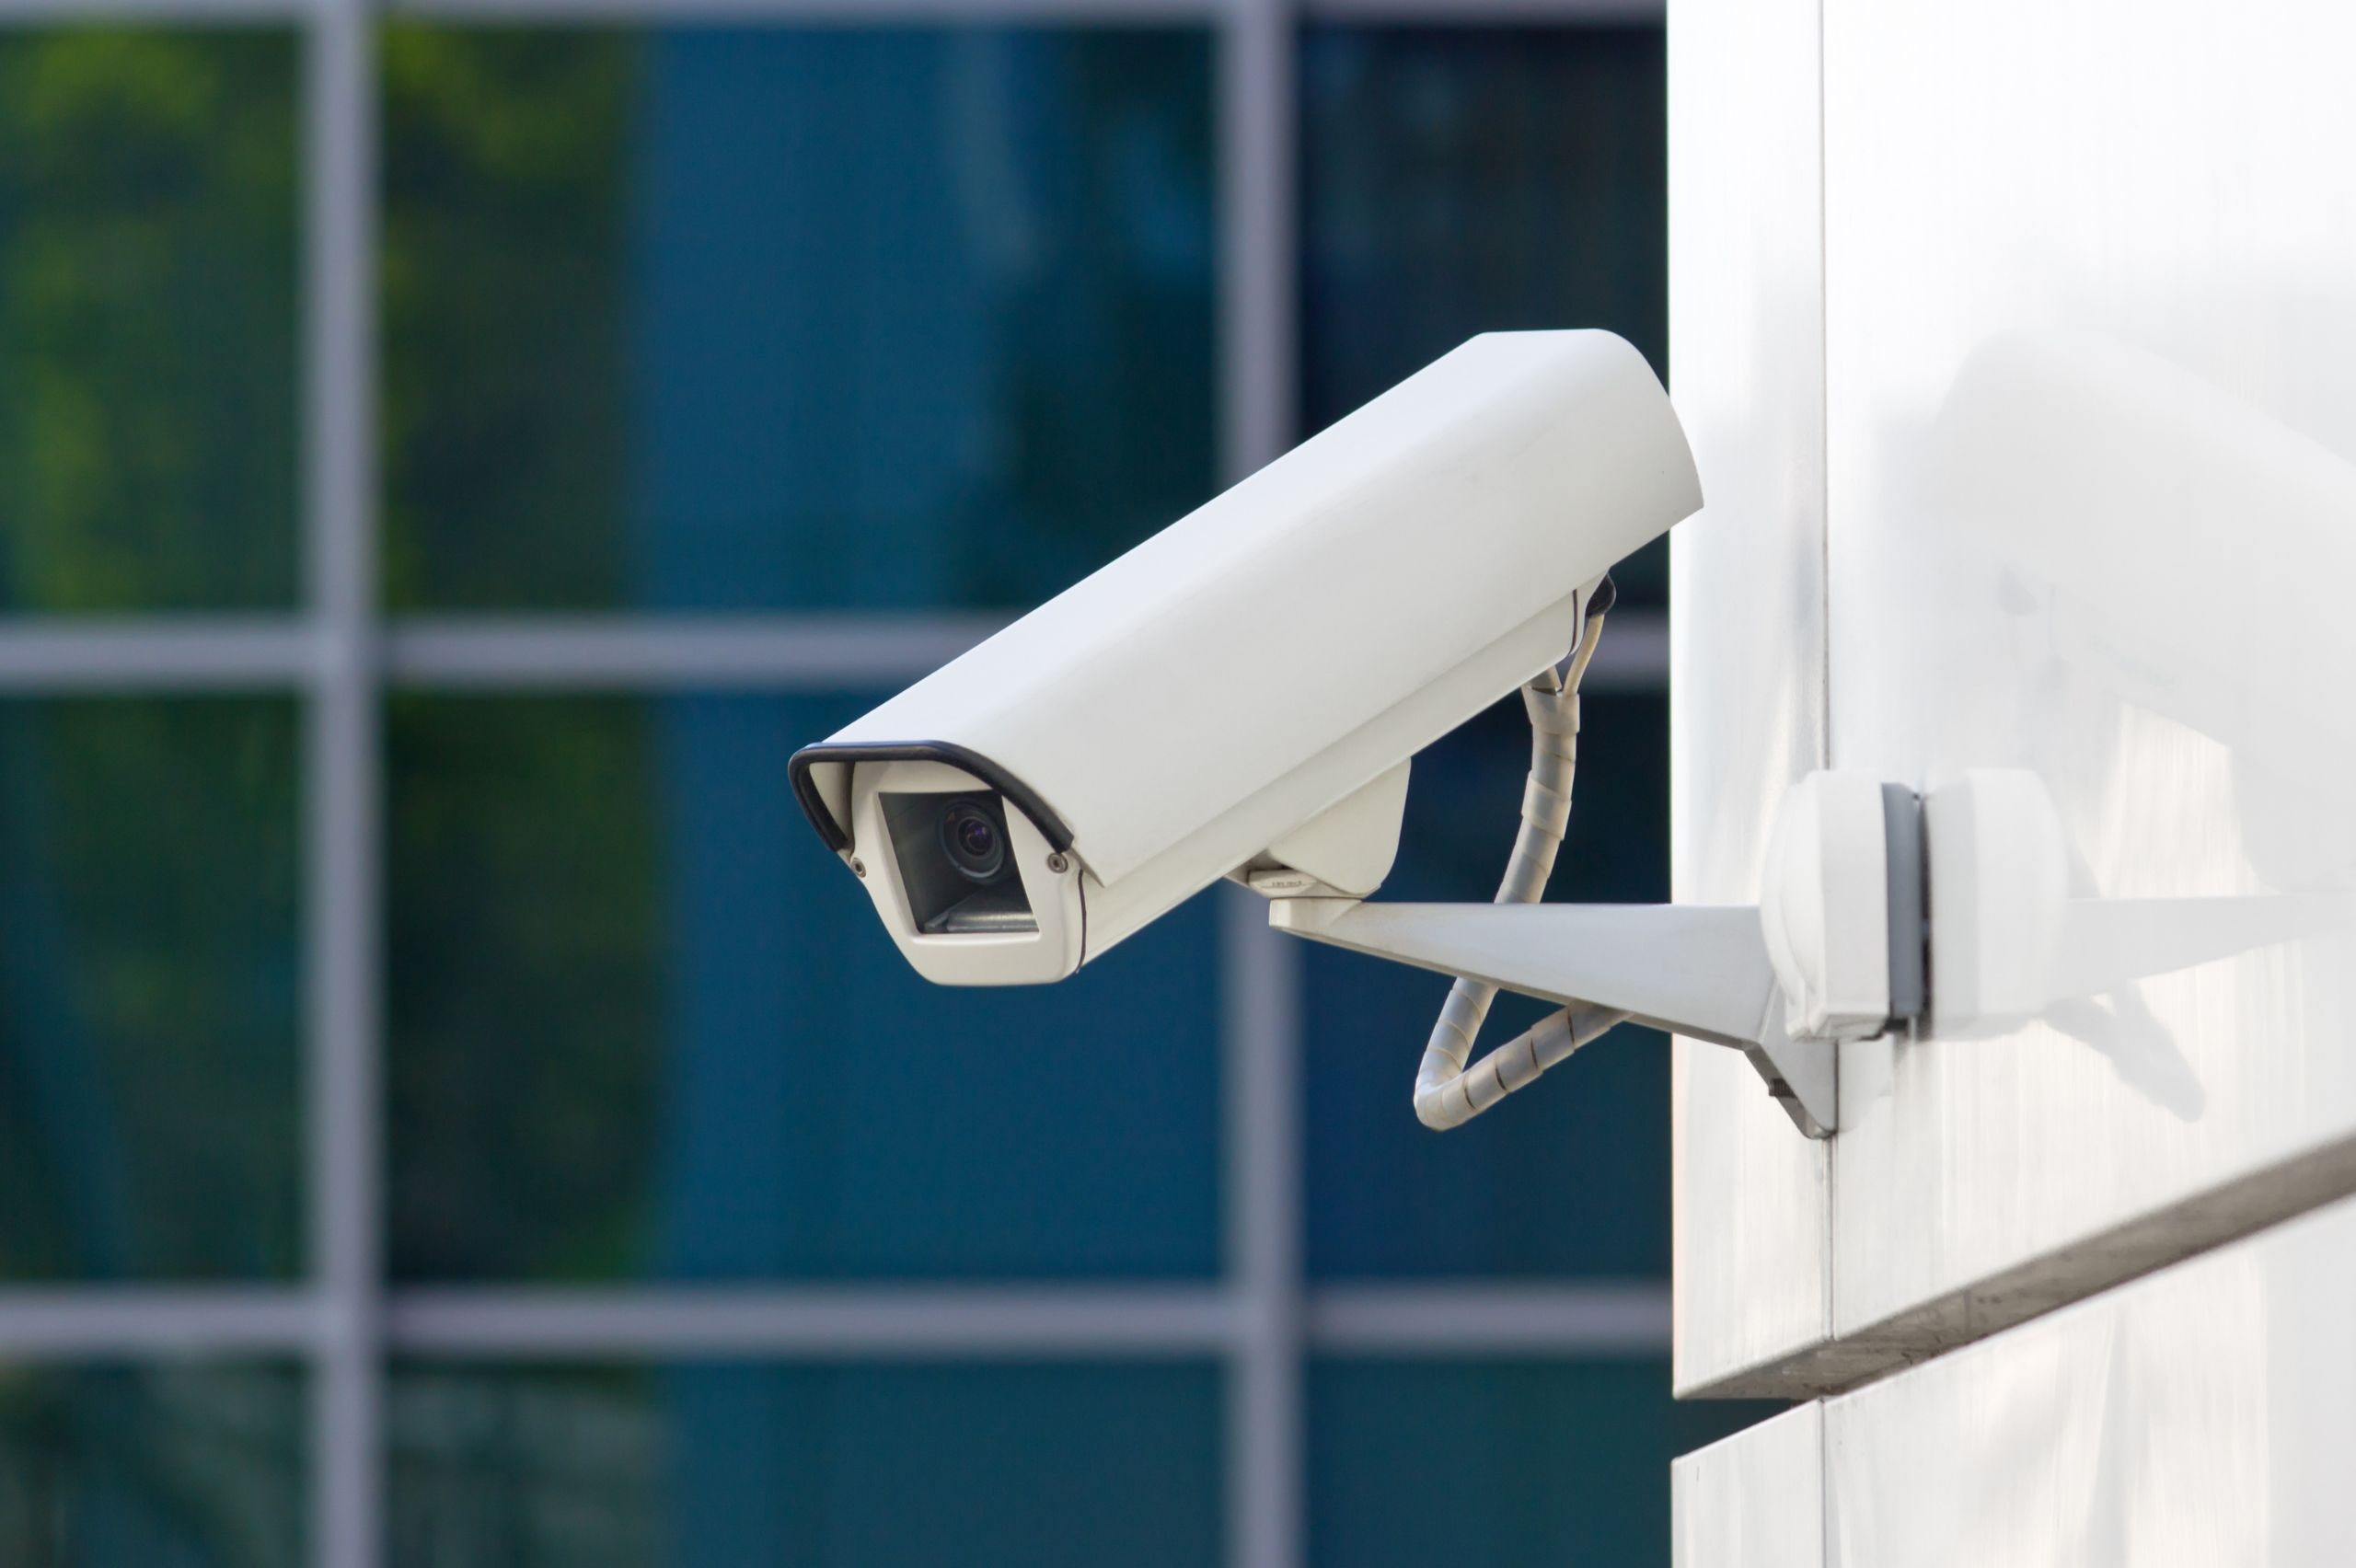
\includegraphics[width=\textwidth]{figs/overt2.jpg} % Include the image
        \caption{Covert cameras}
        \label{fig:covert}
    \end{minipage}
\end{figure}

\selectlanguage{english}\citet{rfc42} identified a spectrum of problems in control room environments, 
specifically in the management and operation of \ac{cctv} systems. A critical aspect is the 
poor technology configuration in these environments, which includes improperly positioned cameras in 
low-crime zones or areas with blind spots, and the adverse effects of weather on analog signals. Additionally, 
outdated or malfunctioning equipment, like broken camera controllers, further impairs surveillance effectiveness. 
Also, the quality of video recordings was another area of significant concern. Many control rooms recorded footage at 
low resolutions, rendering it ineffective for detailed analyses or criminal investigations.

\citet{rfc46} proposed a model which delineates a community's surveillance blueprint, marking the prime locations for \ac{cctv} installation. 
\begin{itemize}
    \item Red dots represent primary entry and exit points, ensuring close monitoring of individual movements through these areas;
    \item Black dots are placed at street intersections and corners, providing broad surveillance coverage.
\end{itemize}

In the model described in figure \ref{fig:cctv-positions}, the cameras positioned at red dots 
would be pivotal for controlling access points, while those at black dots would enable panoramic monitoring 
of the area, essential for observing multiple streets and deterring potential criminal activity. 

\begin{figure}[h]
    \centering 
    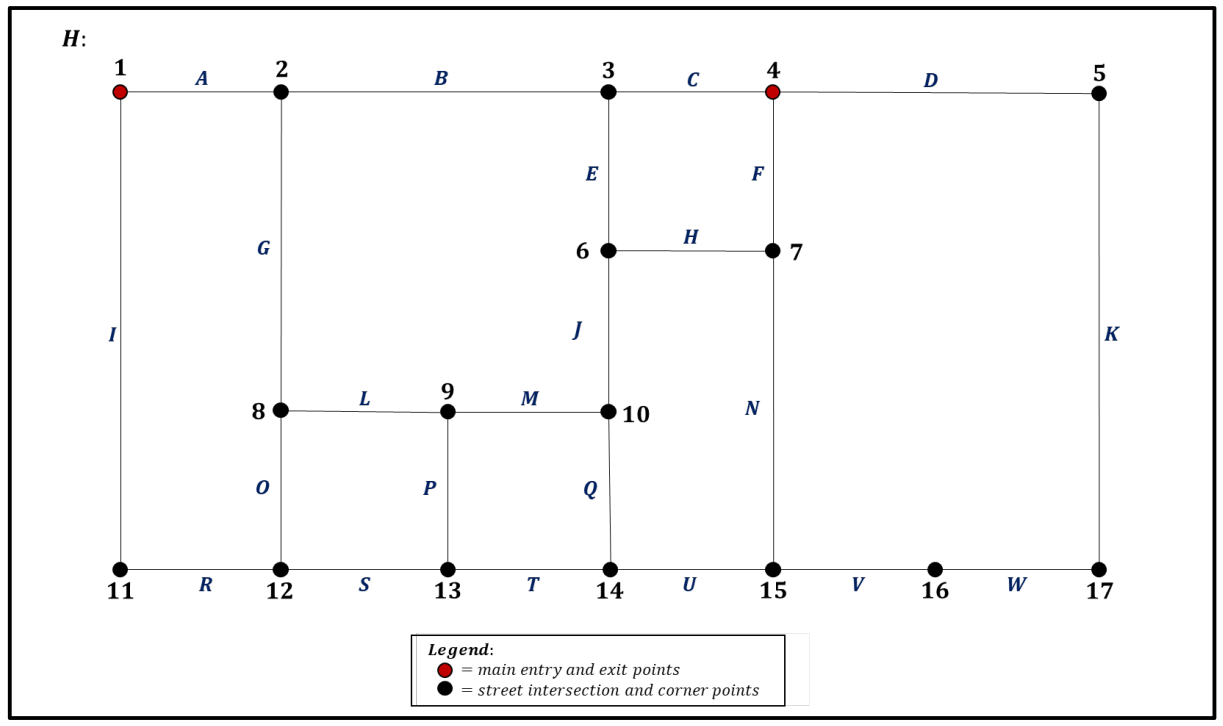
\includegraphics[width=0.75\textwidth]{figs/cctv-positions.png} 
    \caption{Labeled Graph H (Simple Graph Representation of District 5) \selectlanguage{english}\cite{rfc46}}
    \label{fig:cctv-positions}
\end{figure}

\section{Object Detection}
This section covers the basics of object detection, explaining its definition, exploring different methodologies 
used in the field, and outlining key metrics for evaluating performance.
\subsection{General Concepts}
\selectlanguage{english}\citet{rfc2} describe object detection goal as "to determine where objects are located in a given image (object localization) and which category each object belongs to (object classification)", undertaking the dual challenge of not only locating an object within the visual frame, creating a bounding box around it, but also determining its category. \selectlanguage{english}\citet{rfc9} further reinforce this stating "Object detection is a fusion of object location and object classification task".


Object detection is the process of identifying objects in images and videos. The process of 
detecting these objects is fundamentally rooted in the training of object detection models.
There are several key steps in this crucial training phase:
\begin{itemize}
    \item \textbf{Data Collection}: the purpose of this task is to build a set of images, each showcasing the object 
    in a variety of contexts, including different backgrounds and angles;
    \item \textbf{Labeling}: this task aims to annotate (manually or automatically) each image with labels that reflets 
    the object classes, such as the presence of a certain type of object;
    \item \textbf{Feature Learning}: enable a trained model to recognize unique object features such as shape, color, 
    texture, and patterns, these characteristics must be learned. This task is performed using labeled images 
    (the outcome of the previous task);
    \item \textbf{Generalization}: the goal of this task is the generalization of object detection, not only for 
    labelled images, but also for new (unseen) images. A set of metrics make up this task to allow for accuracy 
    when training on unseen objects (images or not). 
\end{itemize} 

\begin{figure}[h]
    \centering 
    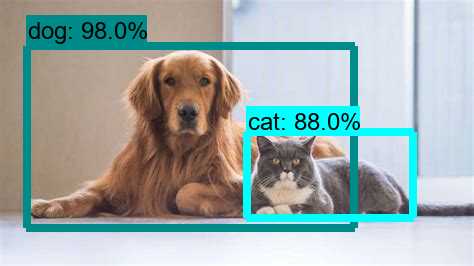
\includegraphics[width=0.5\textwidth]{figs/object-detection.png} 
    \caption{Object Detection Image~\cite{rfc15}}
    \label{fig:object-detection}
\end{figure}

\subsection{Evolution of Object Detection Methods}

The 2014 milestone, figure \ref{fig:stage-detectors}, marks a before-and-after in \ac{ai} applications \selectlanguage{english}\cite{rfc22}. Before, the field predominantly utilized traditional methods for tasks like object detection. These methods involved a multi-step process beginning with the selection of regions in images, which was often inefficient and computationally expensive due to the use of techniques like multi-scale sliding windows. Following this, feature extraction methods such as HOG, Haar-like, and SIFT were employed, but these struggled with variability in backgrounds and lighting conditions. The final step, classification, relied on algorithms like Adaboost, but these traditional techniques frequently fell short in terms of accuracy and efficiency \selectlanguage{english}\cite{rfc9}.

\begin{figure}[h]
    \centering 
    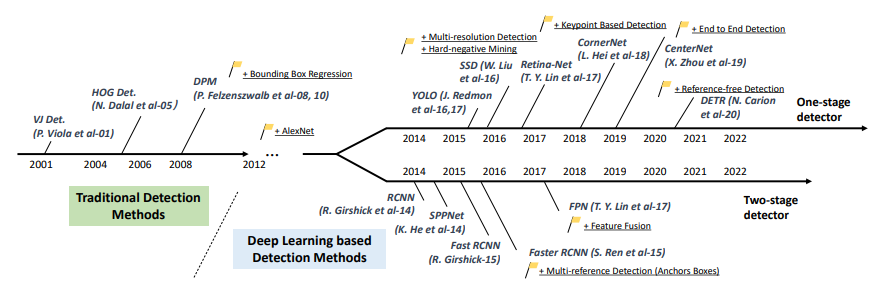
\includegraphics[width=0.97\textwidth]{figs/roadmap-stage.png} 
    \caption{Object Detection Roadmap~\cite{rfc22}}
    \label{fig:stage-detectors}
\end{figure}

After 2014, the landscape of \ac{ai} research underwent a significant transformation with the advent of deep learning-based methods. These new techniques, including \ac{frcnn}, \ac{ssd}, and \ac{yolo}, revolutionized object detection by automatically learning feature representations from data. This shift not only addressed the limitations of the traditional methods, such as high computational costs and inadequate feature representation, but also led to substantial improvements in both the accuracy and efficiency of object detection processes.

As seen in figure \ref{fig:stage-detectors} there are two primary methodologies used for for identifying and 
classifying objects.
These methodologies differ significantly in their operational approach and performance characteristics.

There is the \textbf{two-stage} detection process that operates in a sequential two-phase process. The process involves two key steps: "(i) use a Region Proposal Network to generate regions of interests in the first stage and (ii) send the region proposals down the pipeline for object classification and bounding-box regression"\selectlanguage{english}\cite{rfc21}. The two-stage framework ensures high accuracy but at the cost of speed.

In contrast, \textbf{one-stage} detectors treat object detection as a simple regression problem, directly analyzing the image to determine class probabilities and bounding box coordinates. This approach is faster but generally achieves lower accuracy rates compared to two-stage detectors \selectlanguage{english}\cite{rfc23}.

\subsection{Performance Metrics}
In the field of object detection a variety of metrics are employed to evaluate the performance of detection models. These metrics play a crucial role in both training and testing stages, optimizing classifiers, and measuring their efficiency. 

Precision is calculated as the percentage of correctly identified objects (true positives) among all detections (true and false positives). High precision indicates a low rate of false positives. Recall assesses the model's ability to detect all relevant objects in the dataset. It is the percentage of correctly detected objects (true positives) among all actual objects (sum of true positives and false negatives). High recall implies that the model is effective in identifying most of the relevant objects \selectlanguage{english}\cite{rfc25}.

Following this, accuracy measures the overall correctness of the model, reflecting the proportion of all true results (true positives and true negatives) against the total number of cases.

The \ac{ap} metric integrates precision and recall at different confidence thresholds. It addresses the trade-off between precision and recall, considering detections above a confidence level. \ac{ap} is calculated based on the area under the precision-recall curve \selectlanguage{english}\cite{rfc25}. \ac{map} averages the \ac{ap} across all classes within a database, crucial for assessing multi-class detector performance \selectlanguage{english}\cite{rfc24}. 

F1 score is used to estimate the balance between recall and precision. It is particularly valuable in situations where there is an imbalanced class distribution, as it provides a single metric that combines both precision and recall. Is defined as the harmonic mean\footnote{type of average that gives equal weight to both precision and recall, unlike the arithmetic mean which can be disproportionately influenced by high values of one metric over the other} of precision and recall, \ref{eq:f1score}. 

\begin{equation}
    F1 \text{ score} = 2 \times \frac{\text{Precision} \times \text{Recall}}{\text{Precision} + \text{Recall}}
    \label{eq:f1score}
\end{equation}
    
A high F1 score indicates both high precision and high recall. This metric is particularly useful in the context of binary classifiers on unevenly distributed datasets, where it provides a more balanced view of a model's performance compared to using precision or recall alone \selectlanguage{english}\cite{rfc9}.

\ac{iou} measures the overlap between the predicted \ac{bb} and the ground truth \ac{bb}, Figure \ref{fig:iou}. It's calculated as the ratio of the intersection area to the union area of these \ac{bb}s. The resulting \ac{iou} value ranges between 0 and 1, with values closer to 1 indicating more accurate detection. "The IoU, based on the Jaccard Index, measures the overlap between the predicted bounding box and the ground-truth bounding box." \selectlanguage{english}\cite{rfc24}.

\begin{figure}[h]
    \centering 
    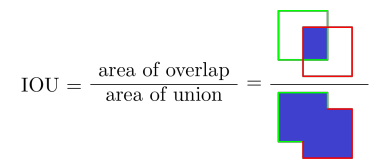
\includegraphics[width=0.5\textwidth]{figs/iou.png} 
    \caption{Intersection over Union \selectlanguage{english}\cite{rfc25}}
    \label{fig:iou}
\end{figure}

\subsection{Algorithms and Techniques Reviews}
This section analyzes current object detection algorithms and methodologies, drawing on a range of studies and 
innovations from various online repositories and databases. It focuses on selected 
reviews\footnote{comprehensive overview or evaluation of existing literature on a particular topic} 
that detail their development, methodologies, outcomes, and contributions to the advancement of object 
detection. This analysis provides insights into the evolution of object detection techniques from their 
inception to modern applications.

\selectlanguage{english}\citet{rfc2} provide a review of deep learning-based object detection methods, 
beginning with the historical context of deep learning and the rise of \ac{cnn}. The review 
covers key models such as R-CNN, which uses selective search for region proposals and \ac{cnn}s for feature extraction, and 
its successors SPP-net, Fast R-CNN, and \ac{frcnn}, which enhance efficiency and accuracy through integrated region 
proposal networks and streamlined processing pipelines. \ac{yolo} introduces a real-time detection 
approach by treating detection as a single regression problem, while \ac{ssd} improves 
small object detection by using multiple feature maps at different scales. The authors emphasize that end-to-end 
training frameworks like \ac{frcnn} significantly boost performance and efficiency, while multi-scale approaches 
like \ac{ssd} effectively address the challenge of detecting smaller objects.

\selectlanguage{english}\citet{rfc8} provide a comprehensive review of image processing techniques, 
emphasizing machine learning applications in visual interpretation. The study begins by highlighting the 
foundational aspects of computational vision, particularly the significance of array-based media computation 
in the digital era. It then examines key image processing algorithms, including \ac{ssd}, \ac{frcnn}, and \ac{yolo}, 
detailing their architecture, methodologies, and distinguishing features. The researchers conduct systematic experiments 
using datasets like Microsoft COCO~\cite{rfc16}, comparing these algorithms to elucidate their respective strengths and 
limitations.

\selectlanguage{english}\citet{rfc9} emphasize the intricacies of computer vision in their review, highlighting 
the significant impact of \ac{dcnns}. Their study spans various applications, from video processing to speech 
recognition, with a particular focus on object detection's importance in areas like transportation and security. 
They detail crucial evaluation metrics, especially \ac{ap}, for assessing detection effectiveness. Notably, they 
mark the pivotal shift to deep learning techniques post-2014, analyzing frameworks like \ac{ssd} and \ac{yolo}. 
By comparing these newer methods with traditional ones and evaluating their performance on datasets like 
PASCAL VOC~\cite{rfc27} and MS COCO~\cite{rfc16}, they offer insights into the dynamic field of object detection.

\selectlanguage{english}\citet{rfc10} review \ac{dl}, highlighting its rapid growth and superior 
performance in various 
fields such as cybersecurity, NLP, bioinformatics, robotics, and medical information processing. The review 
focuses on \ac{cnn}s, detailing their evolution from AlexNet to High-Resolution 
Networks and their advantages, such as automatic feature extraction. The authors address challenges in 
\ac{dl}, including the need for large datasets, model interpretability, and overfitting, proposing solutions like 
data augmentation and advanced optimization algorithms. They also discuss the impact of computational tools 
like \ac{gpu} and \ac{tpu} on \ac{dl} performance. The 
review further highlights the diverse applications of \ac{dl}, showcasing its often superior, sometimes 
human-competitive, performance.

\section{Related Work}
In this section, we systematically review various object detection architectures that could be 
adapted/inspired to our approach. 

Therefore, a comprehensive overview of these contributions is presented, organized 
into focused areas: research methodologies, an in-depth comparative analysis of weapon detection technologies, a 
thorough exploration of datasets pertinent to this field, and a review of the various architectural approaches 
employed in weapon detection systems.

\subsection{Research Method}
This section presents a comprehensive review of critical research in the field of weapon detection. 
The review is structured into three key areas: insights from other 
researchers' datasets and system architectures. Due to the wide range 
and variety of articles from different fields, a careful selection method was used. The search, conducted on 
Scopus, ResearchGate, and arXiv, focused on keywords like "deep," "learning," "real," "time," "weapon," and 
"detection." This search initially produced a large number of articles. A detailed and strict selection process 
was then applied to choose the most relevant articles that significantly relate to the main theme, 
resulting in a final count of 16 documents.

\subsection{Analysis of Datasets in Weapon Detection}
The datasets are a crucial element for this kind of tasks, because they mimic real-world situations. Thefore, the 
gathering of datasets is a relevante baseline to achieve valid results in a object detetion task.
In~\citet{rfc3} study, the dataset comprises three distinct classes: short guns, long guns, and knives - Figure \ref{fig:rehman-dataset}. This dataset is gathered from a variety of platforms, including surveillance videos from YouTube, simulations of firearms and knives created within the Unity framework, and images of pistols, revolvers, and knives from the Open Images Dataset as well as Kaggle. For video, a set of individual frames was extracted and manually labeled using the LabelImg Python utility. To enhance the model's training performance, data augmentation techniques were employed.

\begin{figure}[h]
    \centering 
    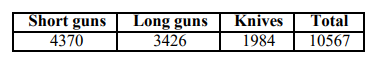
\includegraphics[width=0.45\textwidth]{figs/rheman-dataset.png} 
    \caption{Dataset images classes number~\cite{rfc3} }
    \label{fig:rehman-dataset}
\end{figure}

\selectlanguage{english}\citet{rfc4} developed datasets for real-time weapon detection, focusing on pistols in various settings. Data was sourced from the internet, YouTube, GitHub, research groups, and the Internet Movie Firearm Database \selectlanguage{english}\cite{rfc28}, leading to three datasets categorized into 'Pistol' and 'Not-Pistol' classes, Figure \ref{fig:bathi-dataset}. The 'Pistol' class contained handheld weapons like pistols and revolvers, while 'Not-Pistol' included objects often confused with weapons, like wallets and cell phones. The researchers standardized image size and resolution during data preparation, applied mean normalization, and used data augmentation to enhance the dataset, aiding the model's generalization capabilities.
\begin{figure}[h]
    \centering 
    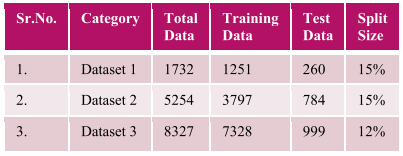
\includegraphics[width=0.45\textwidth]{figs/bathi-dataset.png} 
    \caption{Datasets created by~\cite{rfc4}}
    \label{fig:bathi-dataset}
\end{figure}

\selectlanguage{english}\citet{rfc5} used Google Collab \selectlanguage{english}\cite{rfc26} to train models on 1496 images using \ac{yolo}v3 and \ac{yolo}v5 with pre-trained COCO dataset weights \selectlanguage{english}\cite{rfc16}. The images were divided into 1200 for training and 296 for validation and testing (148 each). Training lasted 40 epochs, taking about 120 minutes, with images sized at 416x416 pixels. Both models, within the PyTorch framework, utilized a COCO pre-trained backbone feature extraction network, which was fine-tuned during training to better represent handguns.

\selectlanguage{english}\citet{rfc6} used a comprehensive dataset consisting of 10014 distinct weapon images 
to train and evaluate the model's accuracy. These images were categorized into three primary object types: knives, 
with a total of 3641 images; long guns, comprising 2497 images; and small guns, which included 3876 images. The 
dataset was strategically divided, allocating 80\% of the images (8011 images) for training and the remaining 20\% 
(2003 images) for testing. Each image used had a resolution of 240 x 240 pixels, and during the training phase, they 
were processed in batches of 32.

\selectlanguage{english}\citet{rfc7} and Moran et al. \selectlanguage{english}\citet{rfc18} both utilized the DaSCI Weapon Dataset \cite{rfc29} for weapon detection research, with \selectlanguage{english}\citet{rfc7} focusing on differentiating weapons from ordinary objects and training their system on 91 weapons. Additionally, employed the CAVIAR Dataset \cite{rfc30} for Suspicious Behavior Prediction, using its video clips of six human actions, annotated in XML, to classify actions as suspicious or not. They parsed XML files to align annotations with video frames for analysis. \selectlanguage{english}\citet{rfc18} used the DaSCI Dataset \cite{rfc29} for knife detection, comprising 2,078 images, primarily from the internet and YouTube. They also utilized the MS COCO 2017 Dataset \cite{rfc16}, a larger dataset with 330,000 images in 80 classes, including 4,326 images labeled under the 'knife' class.

\selectlanguage{english}\citet{rfc17} faced challenges in gathering a comprehensive weapon dataset, particularly for knife and screwdriver images, due to the lack of labeled datasets suitable for classifier training. To overcome this, they used web scraping to gather images from websites and GitHub. These images were manually labeled with tools like LabelImg and Roboflow, and standardized to a 416 x 416 resolution. Their final dataset contained about 6,000 images, with 2,000 each of pistols, knives, and screwdrivers. For training and testing their models, they divided the images in an 80:20 ratio.

\selectlanguage{english}\citet{rfc19} installed a Raspberry Pi B+ with a camera 1.8m high to capture images of consenting students with handgun replicas at a lab entrance. They initially collected 14k images at 1920x1080 resolution, which were expanded to 28k after data augmentation. A challenge in their study was the small size of the guns in the images, posing a risk of misclassification.

\selectlanguage{english}\citet{rfc20} used the ARMAS Weapon Detection Dataset and IMFDB Weapon Detection System \cite{rfc28} for firearm-related crime image collection. The datasets included 3000 and 4940 images of pistols and rifles, respectively. These images underwent preprocessing to fit object detection standards and were split into training and testing sets in an 80:20 ratio.

\subsection{Architectural Approaches in Weapon Detection}
The evolution of real-time weapon detection systems has been significantly influenced by diverse architectural approaches proposed by various researchers. This section delves into a brief analysis of some of these architectures.

\begin{figure}[h]
    \centering 
    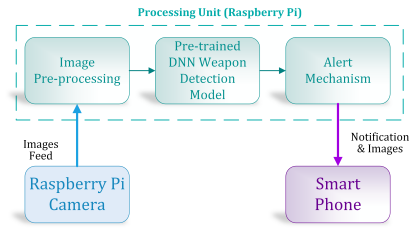
\includegraphics[width=0.36\textwidth]{figs/uob-architecture.png} 
    \caption{\selectlanguage{english}\citet{rfc44} System Diagram}
    \label{fig:uob-architecture}
\end{figure}

\selectlanguage{english}\citet{rfc44} system's operation begins with a Raspberry Pi Camera, which serves as the image capture device, feeding live images into the processing unit, a Raspberry Pi. Once the images are pre-processed, they are fed into a pre-trained Deep Neural Network (DNN) weapon detection model. Upon successful detection of a weapon, the system activates an alert mechanism. Finally, the system sends a notification along with the images of the detected weapon to a smartphone.

One of the standout features of \selectlanguage{english}\citet{rfc6} architecture, Figure \ref{fig:gawade-architecture}, is its integration of an alarm system that activates upon successful weapon detection, thereby ensuring immediate alert to security personnel. This aspect of the model not only enhances its practical application but also significantly contributes to the safety and security in public spaces like malls, airports, and railway stations.
\begin{figure}[h]
    \centering 
    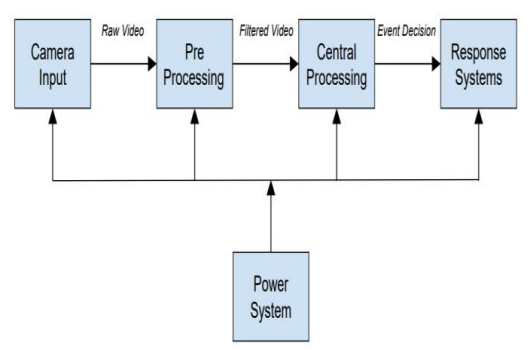
\includegraphics[width=0.4\textwidth]{figs/Gawade-architecture.png} 
    \caption{\selectlanguage{english}\citet{rfc6} Architecure Diagram}
    \label{fig:gawade-architecture}
\end{figure}

\selectlanguage{english}\citet{rfc17} architecture relies on the \ac{yolo}v8 algorithm. The process begins with collecting a large set of images that will be used to teach the detection model what various weapons look like. Each image is then labeled to identify where the weapons are. Once the images are labeled, they are processed to ensure they're in the right format for the model to learn from them effectively. Next, the images are used to train the \ac{yolo}v8 object detection model. Finally, if the system assesses the situation as a medium or high threat, it sends an alert to security guards. This alert includes the image where the weapon was detected and details about the threat level.

The \citet{rfc7} system initiates surveillance and processes the input from two sources: a live webcam and test videos, Figure \ref{fig:shenoy-architecture}. For the live webcam input, the system employs face detection technology to locate human faces within the video frames. If a face is detected, the next step is face recognition, where the system compares the detected face against a database of known criminal records. Simultaneously, the system also runs object detection algorithms to identify potential weapons in the scene. The input from test videos, on the other hand, is fed into a CNN-GRU model. When either the live feed or the test video analysis results in the identification of a criminal, the detection of a weapon or suspicious behavior, the system converges these findings to determine if there's a crime happening. If a crime is detected, the system generates an alert and sends a notification to the concerned authorities.

\begin{figure}[h]
    \centering 
    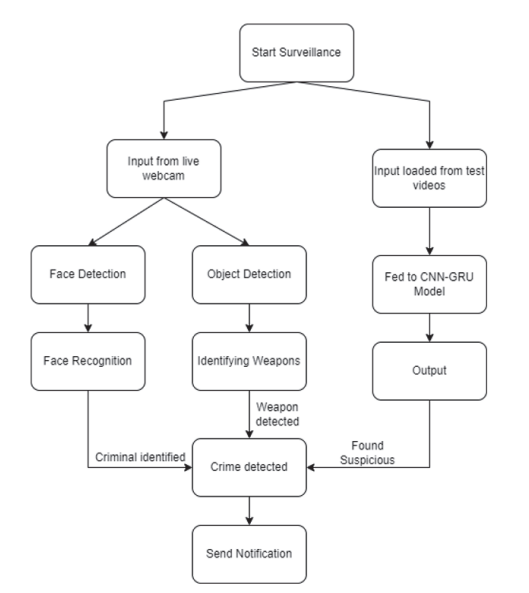
\includegraphics[width=0.6\textwidth]{figs/shenoy-architecture.png} 
    \caption{\citet{rfc7} System Architecture}
    \label{fig:shenoy-architecture}
\end{figure}

\subsection{Comparative Analysis of Weapon Detection Technologies}
\selectlanguage{english}\citet{rfc4} emphasize the importance of security for economic growth and attracting investors and tourists. The study addresses the difficulty of detecting weapons in real-time, considering problems like different angles, blocked views, and hidden weapons. A dataset was adapted by the researchers from diverse sources, including original photos, online repositories, and even film databases. Their exploration spanned several algorithms, like VGG16, Inception variants, and \ac{yolo} iterations. Through rigorous testing prioritizing precision and recall over mere accuracy, \ac{yolo}v4 emerged as the frontrunner, achieving a F1-score of 0.91 and a \ac{map} of 0.92. To illustrate the methodology behind the advanced surveillance techniques discussed, Figure \ref{fig:bhatti-chart} provides a schematic overview of the relationship between object recognition, including classification and localization, and object detection.

\begin{figure}[ht]
    \centering 
    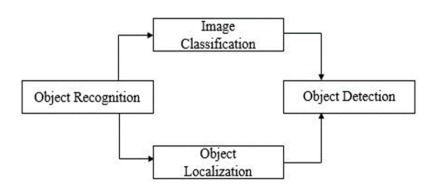
\includegraphics[width=0.43\textwidth]{figs/bhatti-chart.png} 
    \caption{Object recognition to detection hierarchy \cite{rfc4}}
    \label{fig:bhatti-chart}
\end{figure}

\selectlanguage{english}\citet{rfc3} point out the concern of incidents involving firearms and knives due to insufficient security checks. Despite \ac{cctv}s have become prevalent, their constant surveillance demands often surpass human monitoring capabilities. The paper introduces an automated weapon detection system, which employs the \ac{yolo}v5 deep learning model, adapted to a carefully selected dataset. The obtained results achieved a F1 score of 0.95 when applied to \ac{cctv} footage.

In their study, \selectlanguage{english}\citet{rfc5}, address the challenge of detecting concealed weapons in public spaces, despite widespread \ac{cctv} surveillance. They point out the limitations of human monitoring in effectively analyzing extensive footage. To overcome this, they develop an enhanced weapon detection system using the \ac{yolo}v5 deep learning framework, specifically trained on a dataset of 1496 images. This system excels in identifying handguns in various conditions, achieving a \ac{map} of 0.92. Additionally, their comparative analysis with \ac{yolo}v3, as shown in Figure \ref{fig:performance-Thangaraj}, indicates that \ac{yolo}v5 not only improves accuracy in handgun detection but also operates faster and with lower computational demands.

\begin{figure}[h]
    \centering 
    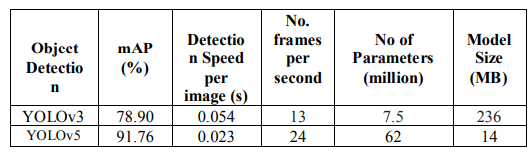
\includegraphics[width=0.55\textwidth]{figs/performance-Thangaraj.png} 
    \caption{Models Performance Comparison \selectlanguage{english}\cite{rfc5}}
    \label{fig:performance-Thangaraj}
\end{figure}

\selectlanguage{english}\citet{rfc18} refers in smart cities context the need for a advanced surveillance applied to urban security. The authors present an approach, combining super-resolution techniques with the \ac{yolo}v4 deep neural network, to detect knives in complex images, a task made difficult by variables like shape, size, and lighting.

\selectlanguage{english}\citet{rfc17}, address the challenge of escalating urban crimes involving firearms and sharp objects in their study. They note the inadequacy of manual monitoring of the extensive data generated by omnipresent \ac{cctv}s in modern cities. To bridge this gap, they have innovated using the \ac{yolo}v8 deep learning framework, tailored to a specialized dataset including images of pistols, knives, and screwdrivers. The system achieved 0.93 accuracy rate on \ac{cctv} footage.

\selectlanguage{english}\citet{rfc6} research tackles the increasingly alarming scenario of weapon-related threats in crowded public spaces like banks, airports, and railway stations. Recognizing that while the deployment of \ac{cctv} cameras has seen a global surge, the sheer volume of footage can overwhelm human operators. This paper introduces a weapon detection system that uses the power of deep learning, specifically through the use of \ac{cnn}. Trained on a dataset of 10014 images, the model adeptly identifies knives, small guns, and long guns, achieving an accuracy rate of approximately 0.85.

In the security system presented by \citet{rfc19}, a key component of the image processing workflow involves the pre-processing of \ac{cctv} feed images to enhance the performance of the deep learning model, Figure \ref{fig:al-mousa-flow}. The system operates by periodically capturing images from \ac{cctv} feeds and analyzing them with a \ac{cnn}, enabling swift identification of potential threats. A distinctive feature of this system is the immediate notification of security personnel via a mobile app, including an image of the detected threat. The system achieves an accuracy rate of 0.92 and can detect threats within 1.6 seconds.

\begin{figure}[h]
    \centering 
    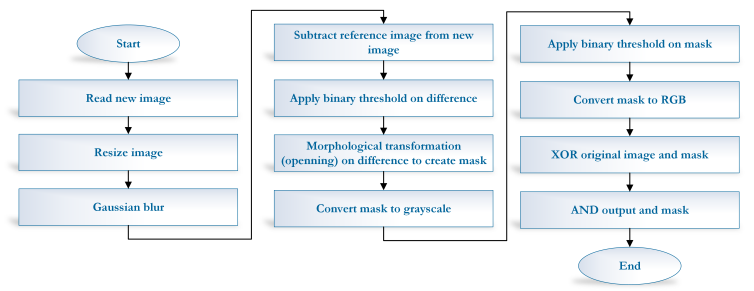
\includegraphics[width=0.65\textwidth]{figs/al-mousa-flowchart.png} 
    \caption{\selectlanguage{english}\citet{rfc19} image pre-processing flowchart}
    \label{fig:al-mousa-flow}
\end{figure}

\selectlanguage{english}\citet{rfc20} address the limitations of \ac{cctv} systems, particularly their dependence on manual monitoring by police personnel, by introducing an automated weapon detection system, Figure \ref{fig:hnoohom-system}. Utilizing two public datasets, ARMAS and IMFDB \cite{rfc28}, their research tests various object detection techniques, including \ac{ssd} MobileNet-V1, EfficientDet-D0, and \ac{frcnn} Inception Resnet-V2. The study highlights the effectiveness of \ac{frcnn} Inception V2 with the ARMAS dataset, achieving a \ac{map} of 0.540, and \ac{ap} scores of 0.793 at 0.5 \ac{iou} and 0.627 at 0.75 IoU.
\begin{figure}[h]
    \centering 
    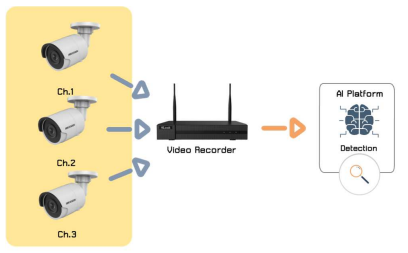
\includegraphics[width=0.37\textwidth]{figs/hnoohom-system.png} 
    \caption{\selectlanguage{english}\citet{rfc20} weapon detection process}
    \label{fig:hnoohom-system}
\end{figure}

\selectlanguage{english}\citet{rfc7} emphasize the alarming rise in criminal activities in urban spaces, despite the ubiquity of \ac{cctv} systems in public areas. Recognizing the limitations of human supervision for these vast surveillance networks, they introduce an intelligent crime detection mechanism. Utilizing the \ac{ssd} Mobilenet architecture fine-tuned on the DaSCI Weapon Dataset \cite{rfc29}, their solution identifies a broad spectrum of weapons, yielding an accuracy rate of 0.81. Moreover, with the integration of the GRU-based behavior analysis model, the system achieved an accuracy of 0.96 in detecting suspicious actions.

Table \ref{models-results} provides a comparative summary of the weapon detection models used by the authors. \ac{yolo} models, particularly \ac{yolo}v5, demonstrate high performance with an F1 score up to 0.95, indicating strong precision and recall. The table also shows that while traditional \ac{cnn} models are effective, with accuracy scores around 0.92, are generally outperformed by the \ac{yolo} series. \ac{frcnn} and \ac{ssd} models show varied results with accuracies ranging from 0.81 to 0.85 and mAP scores as low as 0.54, suggesting they may be less consistent across different datasets. Overall, newer \ac{yolo} models seem to offer a good balance of accuracy and efficiency for object detection tasks.

\begin{table}[ht]
    \centering
    \begin{tabular}{|l|l|l|}
    \hline
    \textbf{Authors} & \textbf{Model} & \textbf{Results} \\ \hline
    \selectlanguage{english}\citet{rfc3} & Yolov5 & F1 Score 0.95 \\ \hline
    \selectlanguage{english}\citet{rfc4} & Yolov4 & F1 Score 0.91, mAP 0.92 \\ \hline
    \selectlanguage{english}\citet{rfc5} & Yolov3, Yolov5 & mAP 0.92 \\ \hline
    \selectlanguage{english}\citet{rfc18} & Yolov4 & - \\ \hline
    \selectlanguage{english}\citet{rfc17} & Yolov8 & Accuracy 0.93 \\ \hline
    \selectlanguage{english}\citet{rfc19} & CNN & Accuracy 0.92 \\ \hline
    \selectlanguage{english}\citet{rfc6} & CNN & Accuracy 0.85 \\ \hline
    \selectlanguage{english}\citet{rfc20} & Faster R-CNN & mAP 0.54, AP 0.79 (0.5 IoU), AP 0.63 (0.75 IoU)  \\ \hline
    \selectlanguage{english}\citet{rfc7} & SSD & Accuracy 0.81 \\
    \hline
    \end{tabular}
    \caption{Authors models and results}
    \label{models-results}
\end{table}

Figure \ref{fig:models-distribution} presents the distribution of different models utilized in previous weapon detection studies, with YOLO models being the predominant choice at 55.6\%, featured in over half of the articles. 

Meanwhile, Figure \ref{fig:metrics-distribution} displays the evaluation metrics that researchers selected for assessing weapon detection models. The Accuracy Rate is the leading metric, employed in 41.7\% of the studies, followed by the F1 Score, which is used in 33.3\% of the cases. The \ac{map} and \ac{iou} metrics are less commonly used, at 16.7\% and 8.3\% respectively.
\begin{figure}[h]
    \centering

    % Image 1
    \begin{minipage}{0.4\textwidth}
        \centering
        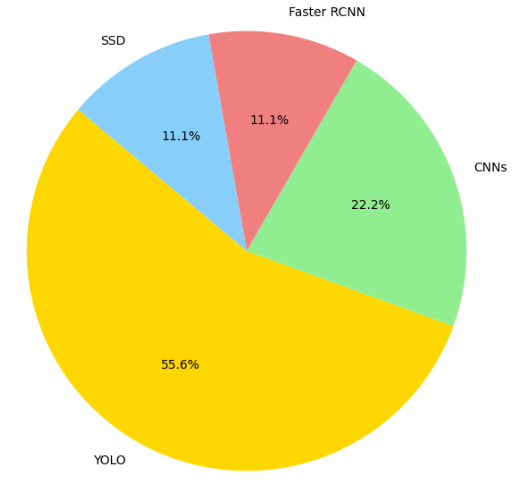
\includegraphics[width=\textwidth]{figs/models-distribution.png} % Include the image
        \caption{Distribution of models used in studies}
        \label{fig:models-distribution}
    \end{minipage}
    \hfill
    % Image 2
    \begin{minipage}{0.5\textwidth}
        \centering
        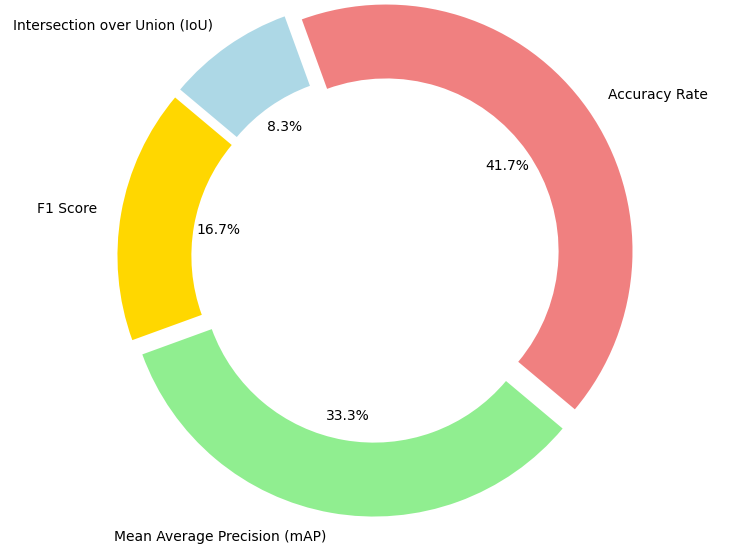
\includegraphics[width=\textwidth]{figs/metrics-distribution.png} % Include the image
        \caption{Distribution of metrics used in studies}
        \label{fig:metrics-distribution}
    \end{minipage}

\end{figure}
\chapter{System Design and Requirements}
\label{chapter:design}

\newenvironment{design}
{\quote\itshape}
{\endquote}

\begin{design}
    This chapter explores the primary architecture that supports the application, outlining its core components and 
    interactions. Also, it covers the basic use cases, along with a comprehensive examination of both 
    functional and non-functional requirements essential for the system's optimal performance.
\end{design}

\section{Basic Use Cases}
The diagram \ref{fig:use-cases} outlines the primary use cases of the application, structured around the user 
interaction flow.

\begin{figure}[h]
    \centering 
    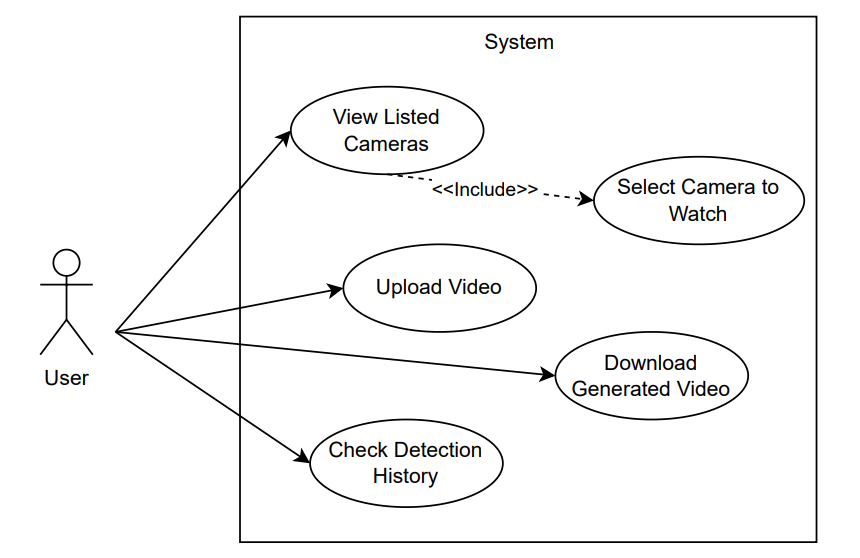
\includegraphics[width=0.6\textwidth]{figs/use-cases3.png} 
    \caption{System Basic Use Cases}
    \label{fig:use-cases}
\end{figure}

At the initial stage, users are presented with a list of all cameras that are registered under their account. 

This list not only displays each camera but also includes information such as the camera's location and current operational
status. Users can conveniently view real-time video streams from these cameras through the application's interface.

Upon viewing the list, users can select any camera to access a more detailed monitoring view. This action 
redirects to a specific page where the video feed from the chosen camera is displayed. This page works 
as the hub for real-time video analysis. While monitoring the video feed, the application actively scans the stream 
for the presence of weapons. If the detection model identifies a weapon within the video, the system generates an alert.

In addition the application supports the upload of pre-recorded videos. Users can upload video files to the platform, which 
are then analyzed by the same detection algorithms used for live streaming.

After uploading a video for analysis, the system processes and annotates the footage with bounding boxes to 
highlight detected weapons. Once the analysis is complete, users have the option to download the annotated video.

Users can also access a comprehensive log of all detection events. This historical data includes detailed information 
about each detection instance, such as the date, time, and frame, enabling users to review past incidents and 
analyze detection patterns over time.

\section{Functional Requirements}
The main goal is to design and implement a real-time weapon detection system capable of 
analyzing surveillance footage and triggering immediate alerts. A prototype showcasing this functionality was developed. 
However, during testing and demonstrations, limitations became evident. Sometimes video streams wouldn't load consistently, 
and alerts were slow to generate. Feedback from security personnel emphasized the need for a more user-friendly 
interface, allowing for quick navigation between cameras and detailed information about detections.

These critical insights guided the development of the core functionalities outlined below:

\begin{enumerate}
    \item Video Stream Handling
    \begin{itemize}
    \item The system shall accept video feeds from various sources, continuously monitoring the video streams 
    and analyze frames for weapon detection;
    \end{itemize}
    \item Detection and Alert Mechanism
    \begin{itemize}
    \item The system shall employ an advanced image recognition algorithm to detect weapons with at least 95\% accuracy;
    \item The system shall generate real-time alerts upon detecting a weapon;
    \item The system shall classify and log each detection event, including time, location, and type of weapon detected;
    \end{itemize}
    \item User Interface
    \begin{itemize}
    \item The system shall offer a user-friendly interface with a dashboard displaying all active video streams;
    \item The interface shall allow operators to navigate easily between different video feeds and alert logs;
    \item The interface shall provide real-time notifications and display detailed information about each detection event;
    \end{itemize}
    \item Data Management
    \begin{itemize}
    \item The system shall store video footage and detection logs securely;
    \item The system shall allow authorized personnel to access and retrieve stored video footage and 
    logs for review and analysis;
    \end{itemize}
    \item Access Control and Security
    \begin{itemize}
    \item The system shall implement user authentication mechanisms to verify the identity of users;
    \end{itemize}
    \item Reliability and Availability
    \begin{itemize}
    \item The system shall include failover protocols to switch to backup systems in case of hardware or software failures;
    \item The system shall monitor its own health and alert administrators to potential issues or failures;
    \end{itemize}
    \item Performance Monitoring
    \begin{itemize}
    \item The system shall continuously monitor its performance, including latency and throughput metrics;
    \item The system shall log performance data and provide administrators with tools to analyze and 
    optimize system performance;
    \item The system shall generate reports on detection accuracy and system performance for regular review.
    \end{itemize}
    \end{enumerate}

\section{High Level Architecture}
Figure \ref{fig:architecture-proposal} illustrates the architecture for the proposed system to 
automatically detect weapons. 

\begin{figure}[ht]
    \centering 
    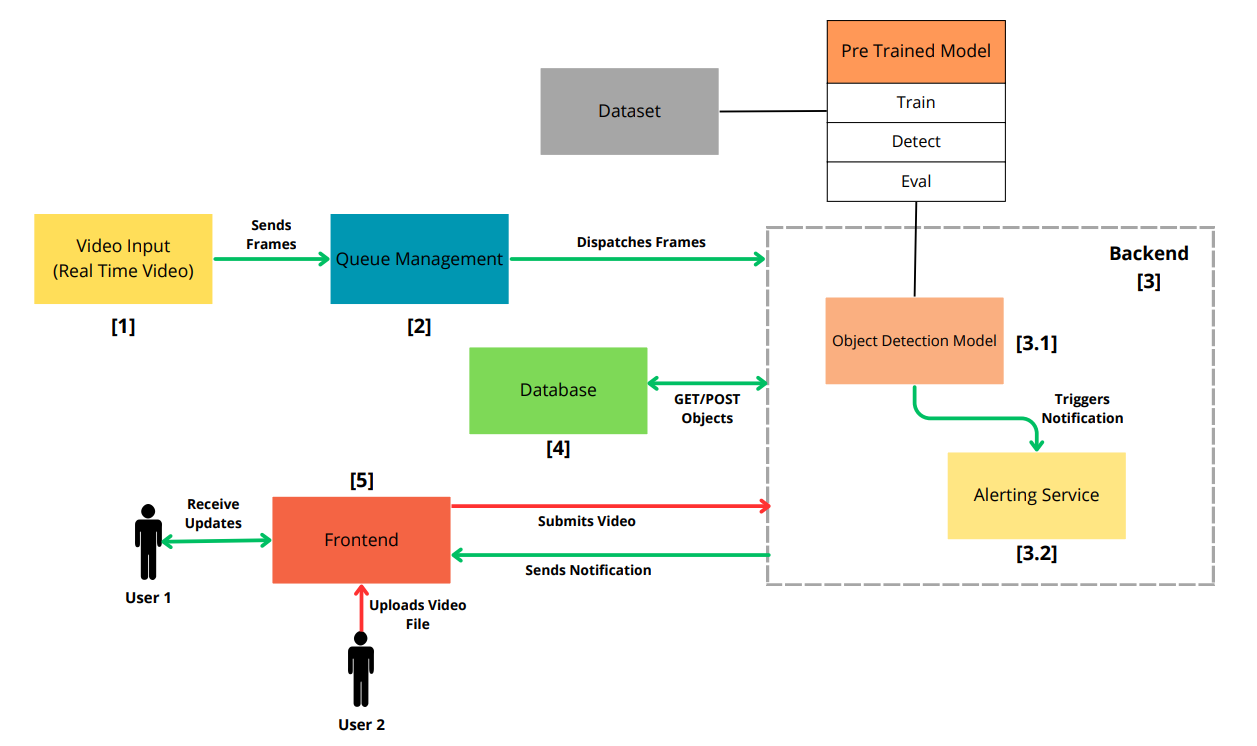
\includegraphics[width=0.95\textwidth]{figs/high-level.png} 
    \caption{High Level Architecture Proposal}
    \label{fig:architecture-proposal}
\end{figure}

% The Video Input (Real-Time Video) [1] consisting of \ac{cctv} cameras strategically installed across various locations, serves as the primary source of video data. These cameras are engineered to capture and transmit real-time video footage, which is then relayed frame by frame to the system for subsequent processing.

The module Video Input (Real-Time Video) [1] aims to feed the system with real-time video using the various \ac{cctv} 
cameras that are spread across various locations.  The video is presented to the system frame by frame, and analyzed 
in the following modules.

% The Queue Management component [2] plays a key role in regulating the incoming data flow. It is specifically tasked with receiving video frames from the \ac{cctv} cameras and systematically queuing them for processing. This component is crucial for several reasons:
The Queue Management component [2] deals with incoming data from previous module, and redeals with incoming data 
from previous module, and regulates the sequence flow. This is a management task, from the balance of received frames 
and sending to futher analysis. Therefore, the following items enumerates the tasks that are associated to this module:

\begin{itemize}
    \item Load Balancing: manages the influx of video frames, particularly crucial during periods of high input. Without this, the backend could become overwhelmed, potentially leading to delays or processing failures;
    \item Prioritization: allows the prioritization of video frames or streams, especially those from high-risk areas;
    \item Scalability: enables efficient scaling without necessitating significant modifications to the backend processing infrastructure.
\end{itemize}

The backend [3] serves as the system's "central processing unit". It is composed by a set of submodules:
\begin{itemize}
    \item Object Detection Model [3.1]: designed to identify objects of interest, primarily focusing on potentially dangerous items like firearms and knives. It operates with a pre-trained model that was trained on a dataset, which has been finely tuned to pinpoint threats with precision.
    \item Alerting Service [3.2]: upon detection of a hazardous object, it promptly generates notifications/alerts. These alerts are then swiftly relayed to the frontend, thereby enabling law enforcement officials to receive real-time updates and respond accordingly.
\end{itemize}

The database [4] stores the critical data gererated by the system, like que video metadata, logs of detected objects, 
model-related data, and other information that supports the system.

Finally, the Frontend [5] enables the interface between system and end users (such as law enforcement officers). Tasks like the uploading of video files for analysis can be performed throw  this interface. Moreover, it serves as a dynamic platform for receiving timely updates and alerts regarding any detected objects, thereby streamlining the communication process and enhancing the efficiency of law enforcement responses.

\section{Non-Functional Requirements}
This section outlines the non-functional requirements essential for the system's successful implementation and operation.
Non-functional requirements define the system's operational attributes, which are crucial to ensuring the system's 
efficiency and effectiveness in real-world scenarios. 

The non-functional requirements can be categorized as follows:
\begin{enumerate}
    \item Performance
    \begin{itemize}
        \item Latency: the system must process video frames with minimal delay to ensure real-time detection;
        \item Throughput: the system should handle multiple video streams simultaneously without significant 
        performance degradation;
        \item Accuracy: high detection accuracy is essential to minimize false positives and false negatives;
    \end{itemize}
    \item Reliability and Availability
    \begin{itemize}
        \item Uptime: the system must maintain high availability, ensuring
        continuous surveillance and monitoring without interruptions;
        \item Fault Tolerance: the system should be resilient to hardware and software failures;
        %\item Accuracy: High detection accuracy is essential to minimize false positives and false negatives. 
    \end{itemize}
    \item Security
    \begin{itemize}
        \item Data Protection: the system must ensure the confidentiality and integrity of video footage. This includes 
        secure data transmission and storage using encryption methods to prevent unauthorized access;
        \item Access Control: strict access control mechanisms should be implemented to restrict system usage to 
        authorized personnel only;
    \end{itemize}
    \item Usability
    \begin{itemize}
        \item User Interface: the system must provide an intuitive and user-friendly interface for 
        operators. This
        includes clear visual indicators for detected threats and straightforward navigation to view 
        video feeds and alerts.
    \end{itemize}
  \end{enumerate}

  \begin{figure}[ht]
    \centering 
    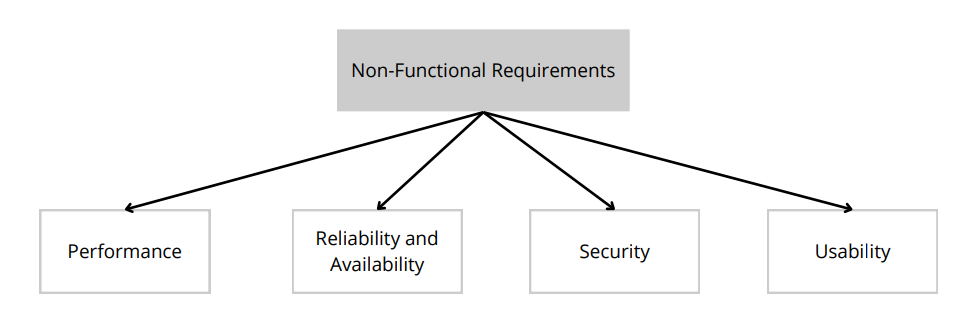
\includegraphics[width=0.65\textwidth]{figs/requirements.png} 
    \caption{Non-Functional Requirements}
    \label{fig:non-requirements}
\end{figure}
%\chapter{SafeGuard System}
\label{chapter:implementation}

\newenvironment{implementation}
{\quote\itshape}
{\endquote}

\begin{implementation}
    In this chapter, the SafeGuard implementation architecture is described, detailing each component and the 
    technology stack utilized, providing a comprehensive overview of how all parts of the system are 
    integrated and work together.
\end{implementation}

\section{Architecture Overview}
\begin{figure}[h]
    \centering 
    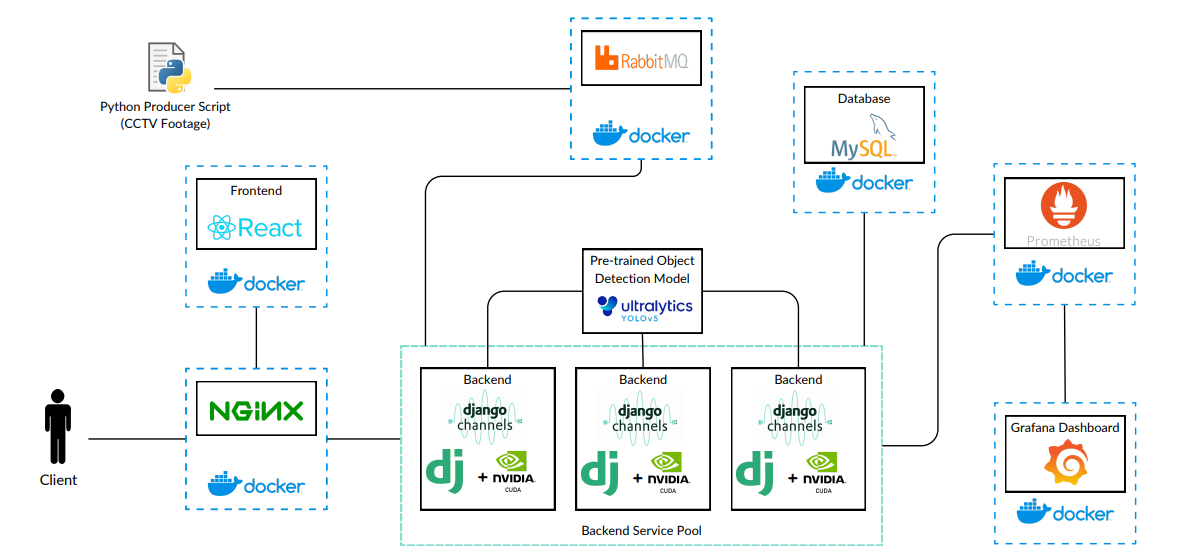
\includegraphics[width=0.95\textwidth]{figs/implementation-architecture6.png} 
    \caption{Implementation Architecture Overview}
    \label{fig:implementation-arch}
\end{figure}
Building this weapon detection system architecture, described in figure \ref{fig:implementation-arch},
 raises several challenges, 
especially integrating a trained model that detects weapons in real time enviroment,
and its large-scale deployment.

First, we developed a Python 3.10 script that simulates the CCTV footage, acting as a producer by sending video 
frames to the next stage (Queue Management), reproducing real-time surveillance.
Because we are dealing with various cameras with different video streams, the Queue Management was built under 
the RabbitMQ \cite{rfc48}, as message broker, which allows to organize video streams into queues
specific to each user, containing the video streams from their respective cameras. This
structure not only helps in managing the video data efficiently but also ensures that each
user's data is handled securely and separately.

The backend of the system is built using Django 5.0.6, chosen for its rapid development and maintainability, 
and employs \ac{gpu}/\ac{cuda} technology to enhance the 
running of detection model inference, a pre-trained \ac{yolo}v5 object detection model, fine-tuned with multiple
hyperparameters.
This component consumes the video data queued in RabbitMQ, 
processing each frame. Acting as the system's backbone, it coordinates both video processing and user 
management. Additionally, it supports user authentication and CRUD (Create, Read, Update, Delete) operations, 
interacting with a MySQL database essential for storing and managing user data and detection logs.

An essential feature of the system is its ability to detect weapons in the video frames. Upon detection, the backend 
uses Django Channels and WebSockets to trigger real-time alerts. These alerts are instantly pushed to the frontend, 
ensuring immediate user notification, which is crucial for prompt response and intervention in 
security-sensitive situations.

To manage client requests efficiently, Nginx, known for its speed and efficiency, has been deployed as a load balancer, 
distributing requests evenly among three backend services.
Each backend service shares the pre-trained model, ensuring consistency and reliability in detection results. 
Nginx's lightweight design minimizes its resource usage, allowing the system to run smoothly, ensuring high 
availability and improved performance of the system.

%The user interface is developed using React 18.0.2 designed to be intuitive and user-friendly, providing users with 
%real-time alerts from the backend, a dedicated page listing all cameras associated with them, and a historical log 
%of all detections. Additionally, there is an upload page where users can analyze past recorded videos.

The user interface is built with React 18.0.2, influenced by the familiarity with React for creating user-friendly web 
apps and also for its flexibility. The interface, designed to be intuitive and user-friendly, 
provides real-time alerts from the backend, a dedicated page listing 
all associated cameras, and a historical log of detections. Additionally, there's an upload page for analyzing past 
recorded videos.

Furthermore, Prometheus and Grafana have been integrated for monitoring and visualization of system performance metrics.
This duo provides a clear picture of how the system is running, allowing for proactive maintenance and real-time 
tracking of system health.  Prometheus collects data on various aspects of the system's performance, and Grafana 
transforms this data into easy-to-understand charts and graphs.

\section{Folder Structure}
This section outlines the structure of the project directories and files, designed to support a modular and 
scalable application, figure \ref{fig:folder-structure}.

The root directory, \textit{project/}, serves as the central hub containing all the subdirectories and 
configuration files pertinent to the project. It includes:
\begin{itemize}
    \item Nginx configuration file
    \item Docker configuration file
    \item Producer script
    \item Backend folder
    \item Frontend folder
\end{itemize}

The \textit{backend/} directory of the project has the server-side logic, developed using the Django framework. 
This setup includes all necessary components of a Django application, including models, views, and 
controllers. These elements handle the business logic and database operations and are located within the \textit{base/} 
folder.
The directory also
contains a \textit{requirements.txt} file, 
crucial for defining all the Python dependencies required for the backend. Additionally, it includes the detection 
model files.

In contrast, the \textit{frontend/} directory focuses on the client-side elements of the application, utilizing React to 
build the user interface. This directory contains the main React components and views. It also includes a 
Dockerfile, which specifies how to build the
Docker container for the React application. 
The components/ subdirectory holds individual javascript files that define specific parts of the user interface.

\begin{figure}[h]
    \centering 
    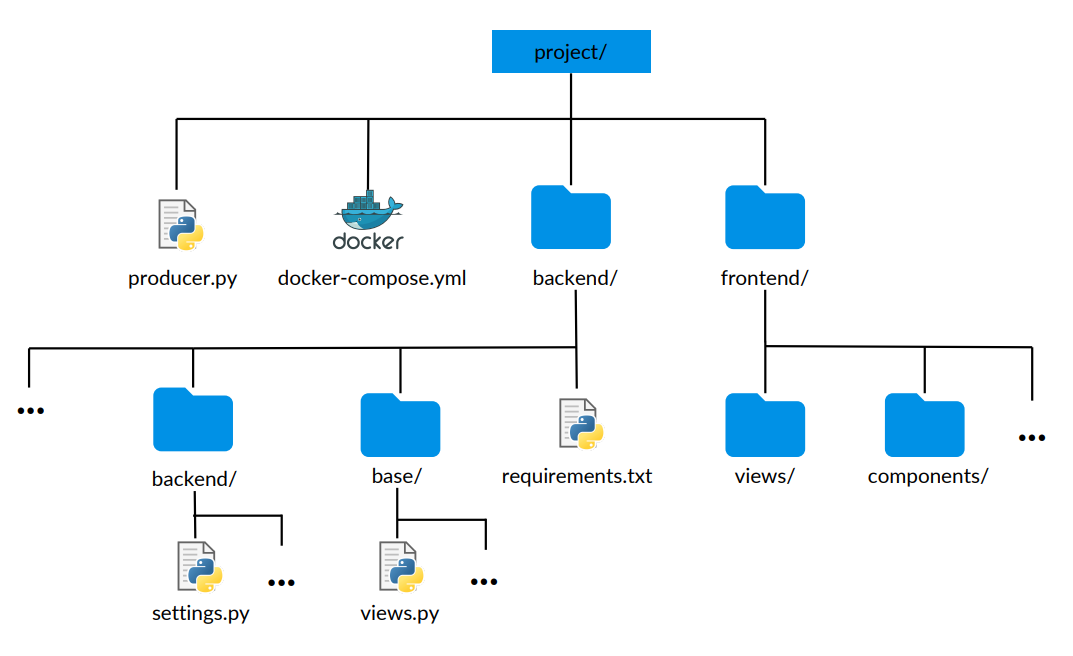
\includegraphics[width=0.7\textwidth]{figs/folder.png} 
    \caption{Folder Structure Diagram}
    \label{fig:folder-structure}
\end{figure}

\section{Video Retrieval and Management}
\subsection{RabbitMQ Setup}
RabbitMQ is a widely adopted message broker that efficiently manages messaging and streaming, making it an ideal 
choice for applications that require robust and scalable message handling. It is 
designed for reliability and flexibility, easily deployed across cloud environments, on-premises, or locally, serving 
millions of users worldwide \cite{rfc48}. Its versatility and reliability make RabbitMQ a fitting backbone for our Django-React 
application, where it orchestrates video data streaming from simulated \ac{cctv} cameras.

To integrate RabbitMQ into our Django-React application, we employ Docker for containerization, which simplifies the 
deployment and scalability of services. The configuration of RabbitMQ within a Docker environment is specified in the 
docker-compose.yml file. Below, are outlined the key settings:
\begin{itemize}
    \item Image: 
        \begin{itemize}
            \item \textit{rabbitmq:3-management} image is used, which includes the management plugin for easy monitoring and management through a web-based interface.
        \end{itemize}
    \item Environment Variables:
        \begin{itemize}
            \item \textit{RABBITMQ\_DEFAULT\_USER} sets the default username.
            \item \textit{RABBITMQ\_DEFAULT\_PASS} specifies the default password.
        \end{itemize}
    \item Ports:
        \begin{itemize}
            \item 5672 is exposed for RabbitMQ server connections.
            \item 15672 is exposed for accessing the RabbitMQ management interface.
        \end{itemize}
    \item Volumes:
        \begin{itemize}
            \item a dedicated volume, \textit{rabbitmq-data}, is used to persist RabbitMQ data and configurations, ensuring data durability across container restarts.
        \end{itemize}
\end{itemize}


\subsection{Message Queuing and Processing}
The message queuing and processing subsystem is crucial for managing the flow of video data from \ac{cctv} cameras to 
the processing backend efficiently, as illustrated in picture \ref{fig:rabbit-mq}. 

RabbitMQ operates by holding, temporarily, messages in queues until they can be safely processed by consumers. 
The setup process involves configuring RabbitMQ queues for each \ac{cctv} camera source. 
These queues store video frames that are encoded as Base64 strings and tagged with metadata: \textit{camera\_id}, 
\textit{user\_id} 
and \textit{timestamp}.

\begin{figure}[h]
    \centering 
    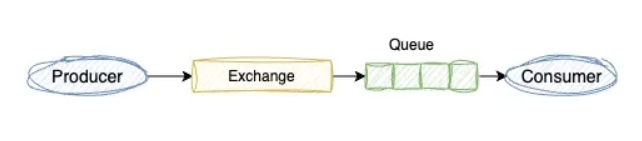
\includegraphics[width=0.5\textwidth]{figs/rabbitmq.png} 
    \caption{RabbitMQ~\cite{rfc48}}
    \label{fig:rabbit-mq}
\end{figure}

The process initiates with each video file from the \ac{cctv} camera being processed frame by 
frame. The OpenCV library \cite{rfc59} is used to capture video frames, which are then encoded into a JPEG format using base64 to 
facilitate easy transmission over the network. Each frame is packaged into a JSON object containing relevant metadata 
and pushed to the designated RabbitMQ queue.

The key function \textit{send\_frame\_to\_queue} is responsible for publishing each frame to its respective queue. 
It constructs a message payload containing the encoded frame and metadata, then sends
this message to the RabbitMQ exchange with a specific routing key corresponding to the queue name.

To enhance the throughput and responsiveness of the system, the video processing operation is executed in multiple 
threads. Each thread handles a different video source, allowing the system to parallelize the workload effectively.
\section{Frontend Development}
\subsection{Views Implementation}
After authentication, user is presented with the first view which lists all the cameras 
associated with their account, as showed in figure \ref{fig:camera-list}. This ensures that users have organized access to 
their specific surveillance resources. 

As mentioned above, the system uses RabbitMQ, which maintains a queue dedicated to each user. When cameras stream video, 
RabbitMQ receives these frames and forwards them to the backend. 
From there, the backend processes these 
frames and sends them to the frontend via WebSockets.

Upon selecting a camera, the user is directed to a second view where the video footage is streamed live, as illustrated in
 figure \ref{fig:camera-page}. 
In parallel, the stream is analyzed using an object detection model. The details of this model, which will be discussed 
subsequently, include the identification of specific objects of interest, in this instance, weapons.

When a weapon is detected, the system triggers an alert that is immediately relayed to the user through a toaster 
notification on the frontend interface. This alert specifies the type of weapon detected and the confidence level 
of the detection, providing information immediately to the user. 

Furthermore, the system ensures that all detections are recorded in a database in real time, thus providing a 
comprehensive and accurate record of events.
This ability to retain data indefinitely permits retrospective analysis, which can prove 
instrumental in both investigative and monitoring activities.

\begin{figure}[h]
    \centering
    \begin{subfigure}[b]{0.49\textwidth}
        \centering
        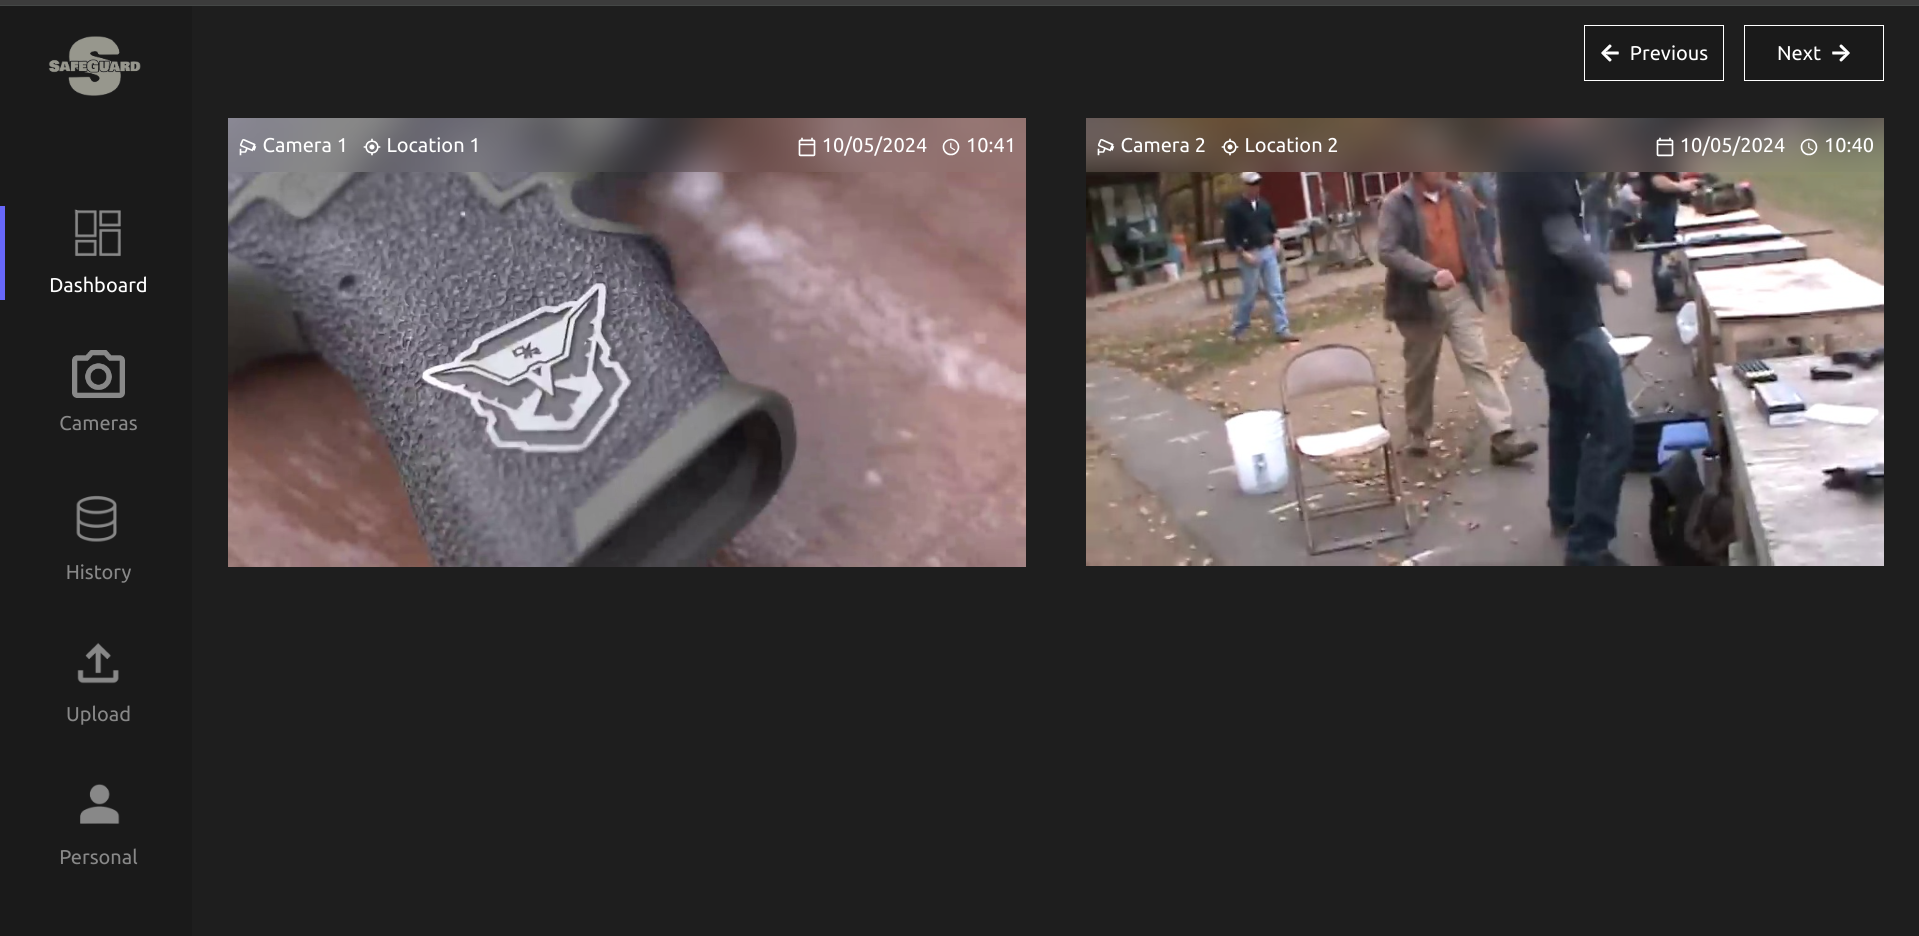
\includegraphics[width=\linewidth]{figs/cameras-list.png}
        \caption{User Listed Cameras}
        \label{fig:camera-list}
    \end{subfigure}
    \hfill % spacing
    \begin{subfigure}[b]{0.49\textwidth}
        \centering
        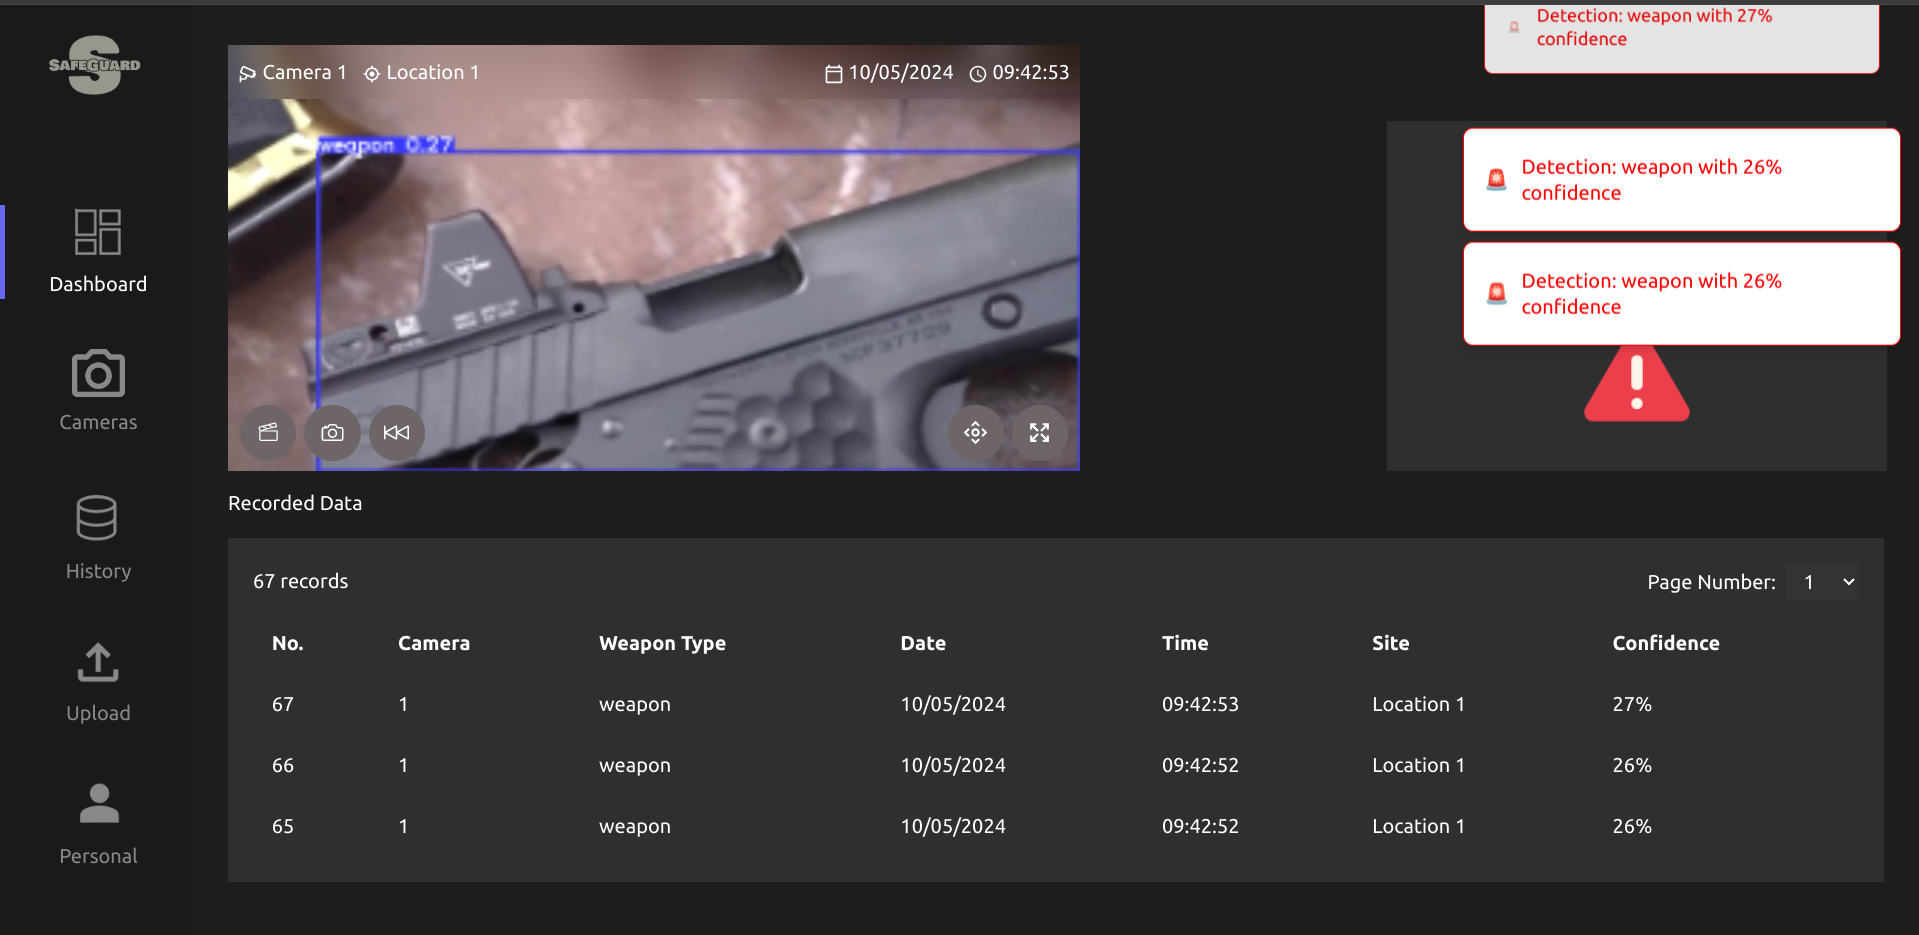
\includegraphics[width=\linewidth]{figs/camera-page.png}
        \caption{Single Camera Analysis}
        \label{fig:camera-page}
    \end{subfigure}
    \caption{Single and Multi Camera Pages}
    \label{fig:cameras-list-camera-analysis}
\end{figure}

Users may access the aforementioned historical data through a History page, as ilustrated 
in Figure \ref{fig:detections-history}, where 
they can view specific instances of detected weapons, including the time of detection and the captured frame.
\begin{figure}[h]
    \centering 
    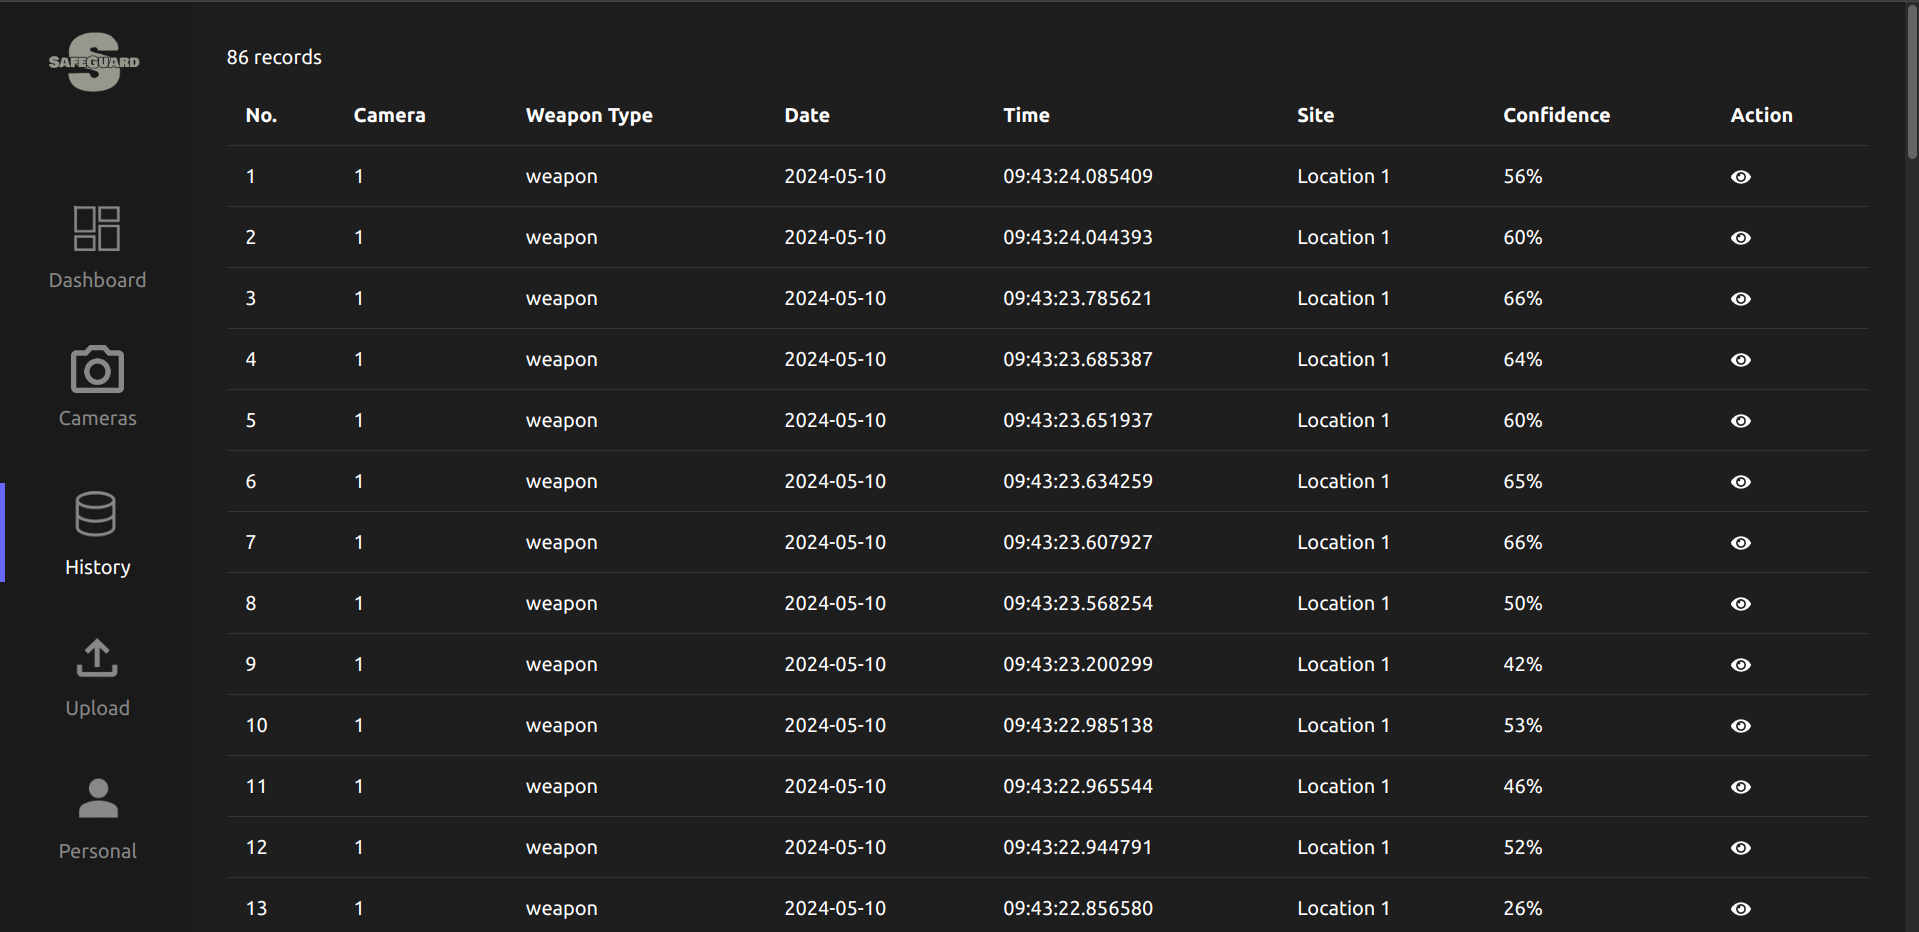
\includegraphics[width=0.65\textwidth]{figs/history-page.png} 
    \caption{Detections History Page}
    \label{fig:detections-history}
\end{figure} 

The application includes a section dedicated to the analysis of pre-recorded videos. This section 
allows users to select and upload a video file in the .mp4 format. %as illustrated in figure \ref{fig:upload-video}.

%\begin{figure}[h]
%    \centering 
%    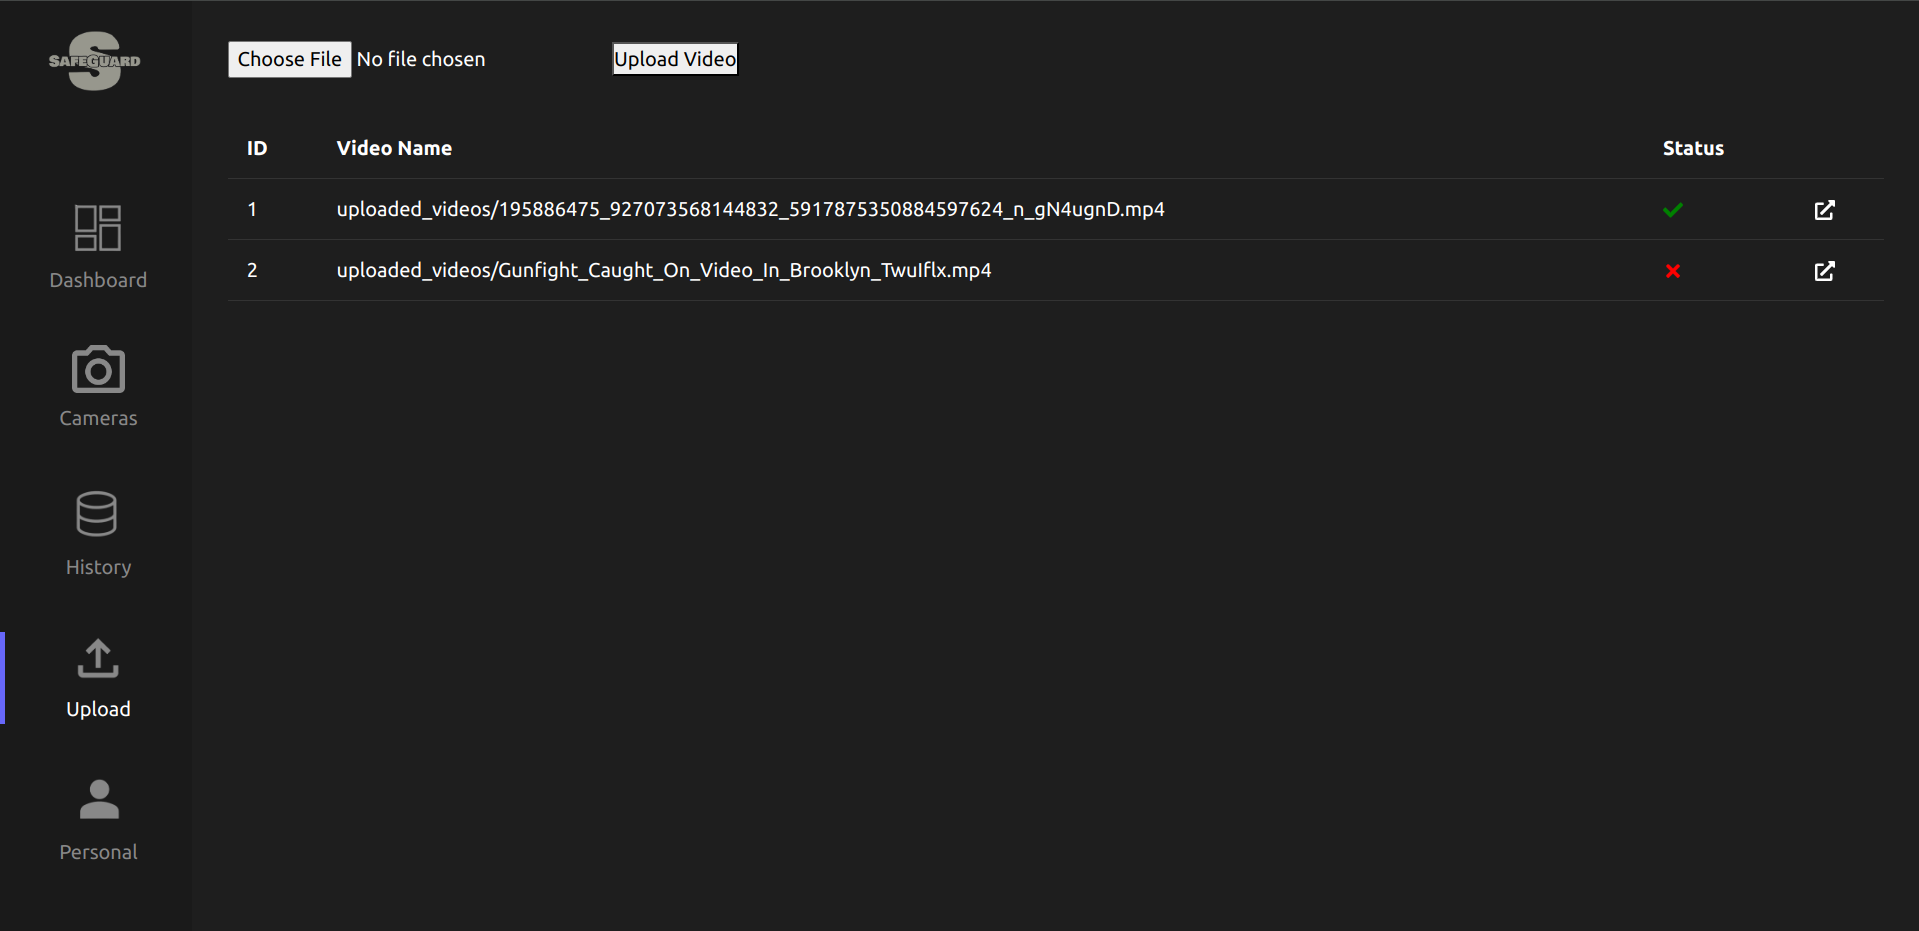
\includegraphics[width=0.65\textwidth]{figs/upload-video-page.png} 
%    \caption{Upload Video File}
%    \label{fig:upload-video}
%\end{figure}

Once a file is uploaded, it appears in a specific list that displays all of the files they have submitted, providing 
users quick access to their uploaded content and enabling them to track the status of each video.

Each file in the list is followed by a status indicator. If a video has not yet been analyzed, its status 
will reflect this, and selecting the video will lead the user to a page where the analysis process begins afresh, 
as ilustrated in figure \ref{fig:upload-video-analysis}. 
Importantly, any previous detections associated with the video are cleared to ensure that the analysis starts from 
the beginning, providing a clean slate for accurate detection. The analysis must run to the completion of the video 
for it to be marked with a check, signifying that it has been fully processed.

For videos that have already been analyzed, users can immediately access and download the processed video, \ref{fig:download-video}. 
The video version presented here includes bounding boxes, drawn around the weapons identified by the system, which 
visually indicate the location and presence of potential threats within the footage. 
Alongside the video, a list of detections are provided in a detailed table. 
This table includes the type of weapon detected, confidence score and the exact timestamp within the video where each 
weapon appears.

\begin{figure}[h]
    \centering
    \begin{subfigure}[b]{0.49\textwidth}
        \centering
        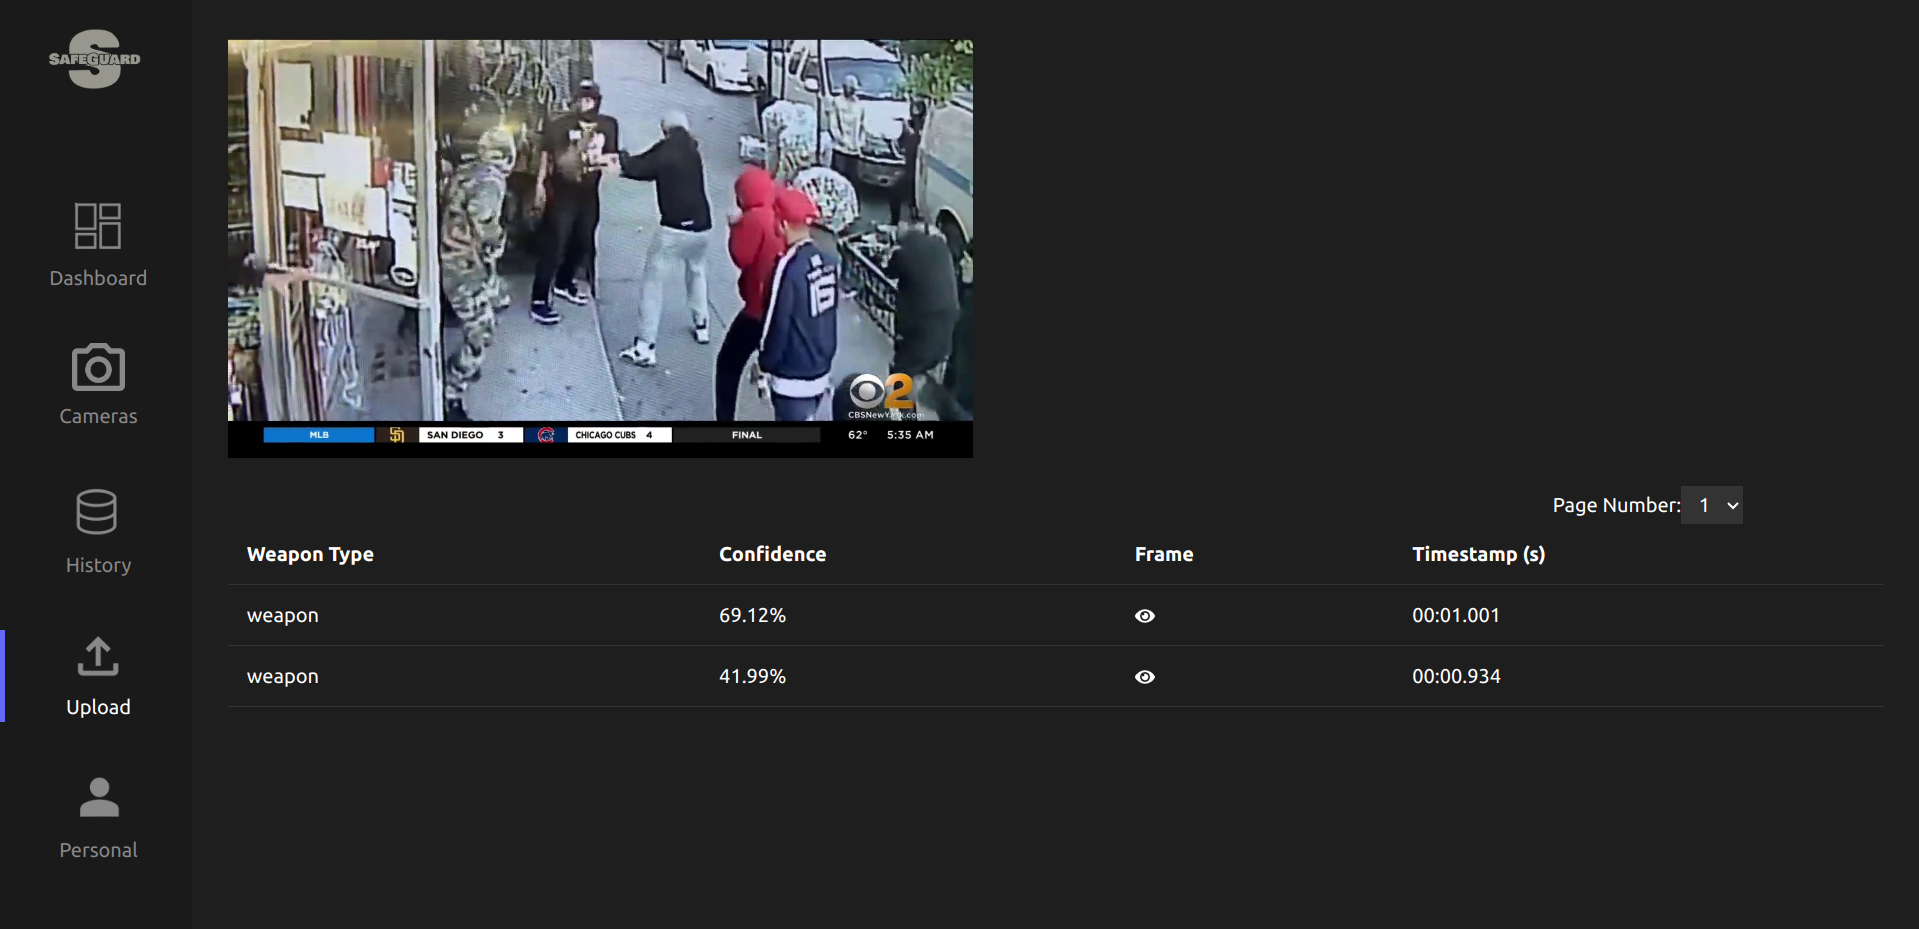
\includegraphics[width=\linewidth]{figs/video-upload-analysis-page.png}
        \caption{Upload Video Analysis}
        \label{fig:upload-video-analysis}
    \end{subfigure}
    \hfill % spacing
    \begin{subfigure}[b]{0.49\textwidth}
        \centering
        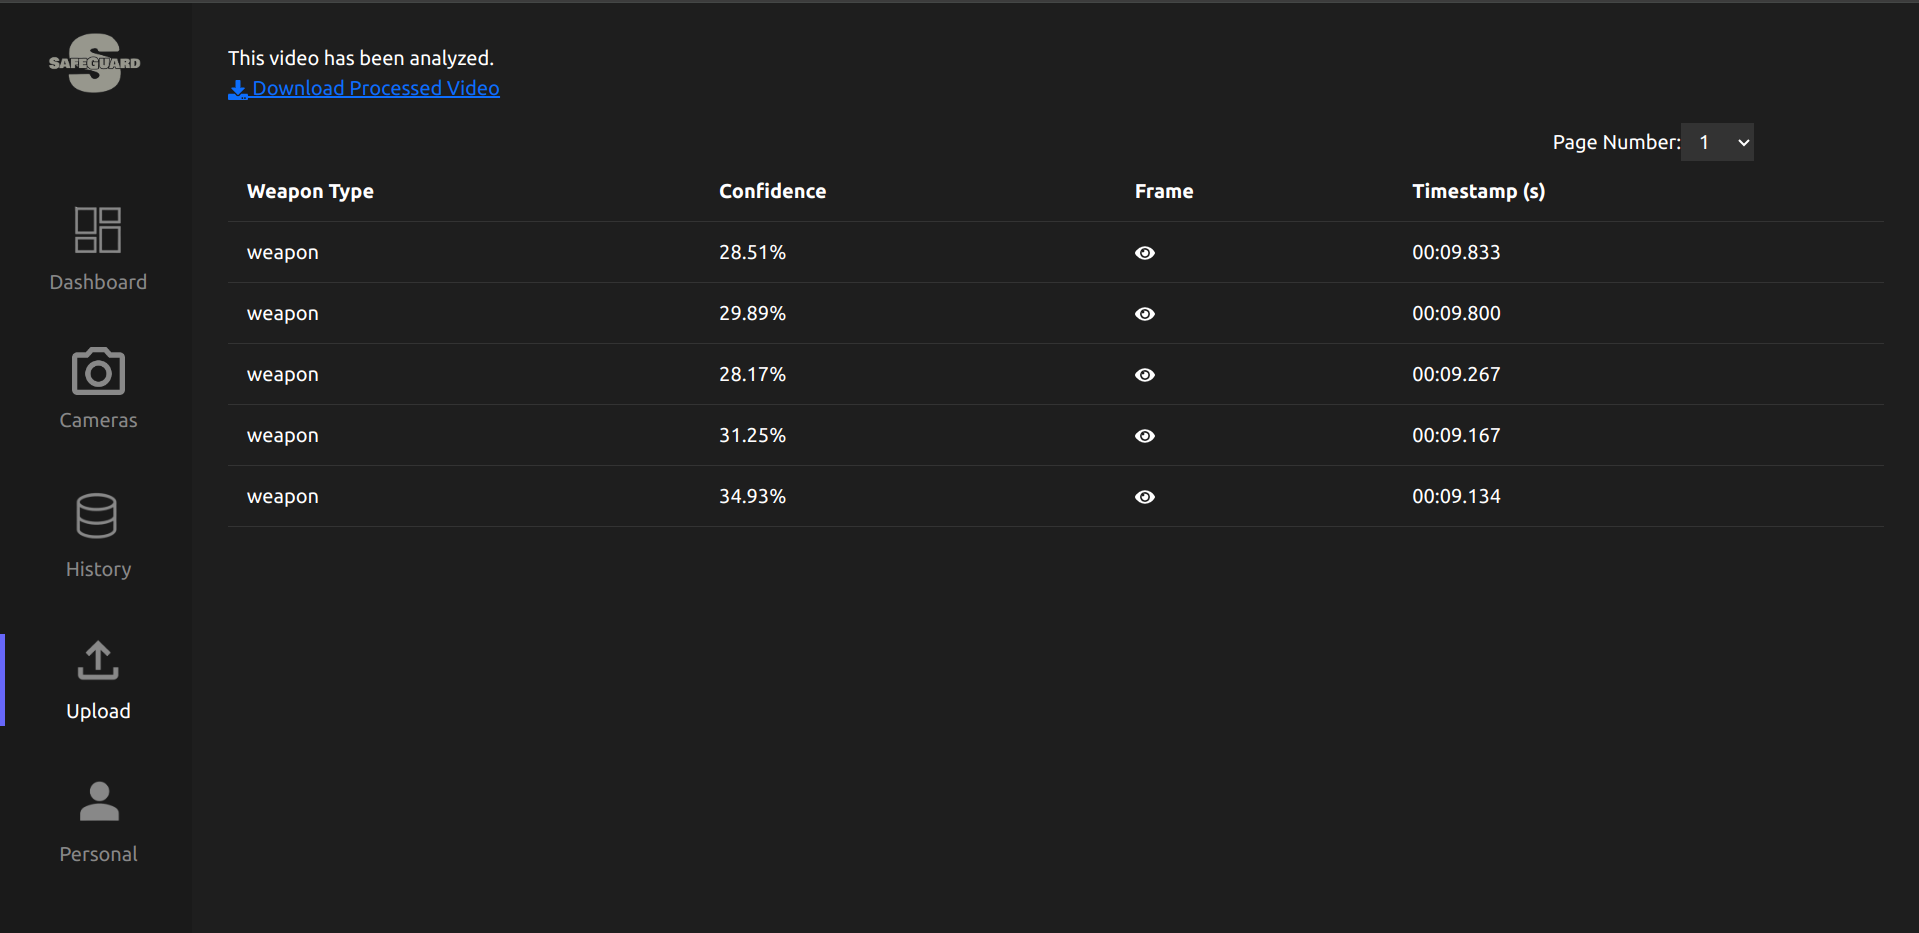
\includegraphics[width=\linewidth]{figs/download-video-page.png}
        \caption{Download Video after Analysis}
        \label{fig:download-video}
    \end{subfigure}
    \caption{Upload Video Feature}
    \label{fig:upload-video-section}
\end{figure}
\subsection{Integration with Docker}
By using Docker, the frontend is encapsulated in a controlled, consistent environment, ensuring that all 
dependencies and configurations are unified across different development and production stages.

The frontend service is built using a Dockerfile 
\footnote{\url{https://github.com/pedromonteiro01/cctv-real-time-weapon-detection/blob/main/project/frontend/Dockerfile}} 
that specifies \textit{node:alpine} as the base image. 
The service configuration includes essential commands to set up the 
working environment, install dependencies, and prepare the service to be run with the \textit{yarn start} command. 
Specifically, the \textit{COPY} commands transfer the necessary project files into the container, and the \textit{RUN} 
command installs all node modules as specified in \textit{yarn.lock}.

This setup facilitates a more efficient development process, allowing for rapid testing and deployment while maintaining 
high reliability and compatibility across various environments. Additionally, the direct transfer of project files 
and dependency management through Docker ensures that the application behaves predictably in every run, reducing 
potential deployment issues.
\subsection{Testing and Quality Assurance}

In frontend development, testing is a critical component that ensures the application is reliable, 
user-friendly, and robust. Three main types of testing have been implemented: unit tests, integration tests, 
and \ac{e2e} tests.

%\begin{figure}[h]
%    \centering 
%    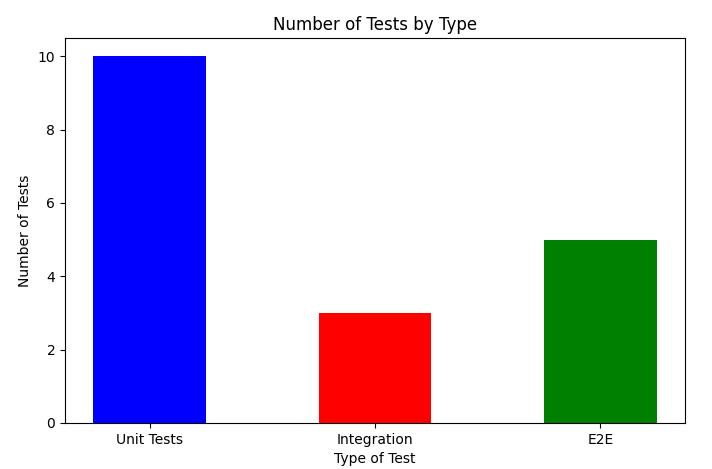
\includegraphics[width=0.5\textwidth]{figs/frontend-tests.png} 
%    \caption{Frontend Types of Tests}
%    \label{fig:frontend-tests}
%\end{figure}

The unit tests were developed using Jest \cite{rfc60} with the main objective to test individual components in isolation. 
This approach focused on ensuring the correct functionality of each component, examining internal logic, state 
management, and behavior under various conditions.

Integration tests were also conducted using Jest. These tests are crucial for assessing the interactions between 
connected components and services. The focus here was on the data flow and state management across components.

For \ac{e2e} testing, was used Selenium \cite{rfc61} with the Firefox driver \cite{rfc62} to simulate real user interactions from start to finish. 
This testing ensures the system behaves as expected in a production-like environment and includes several specific 
scenarios:

\begin{itemize}
    \item Login Test: ensured that authentication works correctly 
    and the user gains access to their account (code listing \ref{lbl:login-test-code});
    \item Upload Video File for Detection: tested the upload of a video file for 
    analysis, ensuring the application handles file uploads and data processing accurately;
    \item Download Analysed Video File: ensures users can download the processed video files, 
    confirming that the files are accessible;
    \item Get User Cameras List: verify that the application could correctly interact with the backend to 
    display the list of the user's connected cameras.
\end{itemize}

Below is an excerpt of the login test, code listing \ref{lbl:login-test-code}.

\begin{listing}[h]
    \begin{minted}{python}
    try:
        driver.get('http://localhost:3000/login') 
        driver.find_element(By.NAME, "username").send_keys("pmapm@ua.pt")
        driver.find_element(By.NAME, "password").send_keys("password")
        driver.find_element(By.CSS_SELECTOR, "button[type='submit']").click()

        time.sleep(5)

        if driver.current_url == 'http://localhost:3000/personal':
            print("Login successful")
        else:
            print("Login failed")
    finally:
        driver.quit()
    \end{minted}
    \caption{Login Test.}
    \label{lbl:login-test-code}
    \end{listing}

The login test navigates to the login page, inputs the 
username "pmapm@ua.pt" and 
password "password", and submits the form. After waiting for 5 seconds, it checks if the URL is 
http://localhost:3000/personal to verify if the login was successful. Finally, it closes the web driver.


\section{Backend Development}
\subsection{Authentication and Security}
This section explores the authentication and security mechanisms implemented in the backend. 
To manage the users of the application, a custom user model was defined, having key attributes such as email, 
names, and password. 

\begin{figure}[h]
    \centering 
    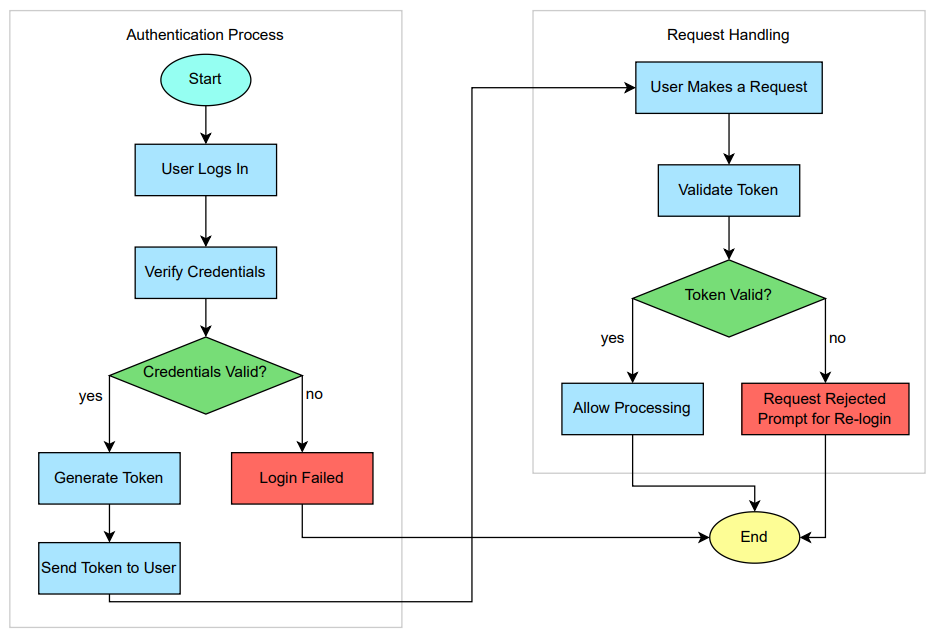
\includegraphics[width=0.75\textwidth]{figs/flow-chart.png} 
    \caption{Authentication Flowchart}
    \label{fig:auth-flowchart}
\end{figure}

Following the flowchart \ref{fig:auth-flowchart}, when a user successfully logs into the system using their credentials (email and password), the backend 
verifies these credentials against the stored data. If the credentials are correct, the server generates a token. 
This token acts as a stand-in for the user's credentials during future requests, thus avoiding the need to resend 
the password over the network, which could be intercepted. Each token is unique and tied specifically to one user.

Once the token is generated and sent back to the user's client, a web browser, it is stored locally, in local storage. 
Every subsequent request will include this token in the request headers, to tell the server which user is making 
the request.

Upon receiving a request that includes a token, the server first validates the token. This validation process checks 
if the token is valid, has not expired, and is linked to an actual user account. If any of these checks fail, 
the server will reject the request.

If the token is valid, the system allows to process the request coming from the user.

For added security, tokens are configured to expire after a certain period. This limits the time an attacker has to 
use a stolen token. When a token expires, the user must log in again, and a new token is generated.

\subsection{Client-Server Interaction Flows}
The system interactions between the client and server, described in figure \ref{fig:flows}, are divided 
into two main processes, each supporting a different aspect of video management and surveillance. 
\begin{figure}[h]
    \centering
    \begin{subfigure}[b]{0.45\textwidth}
        \centering
        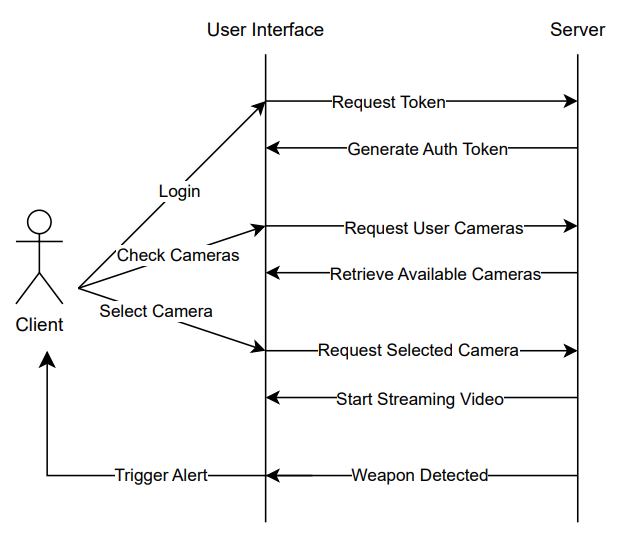
\includegraphics[width=\linewidth]{figs/flow1.png}
        \caption{Real-time Camera Detections Flow}
        \label{fig:flow1}
    \end{subfigure}
    \hfill % spacing
    \begin{subfigure}[b]{0.45\textwidth}
        \centering
        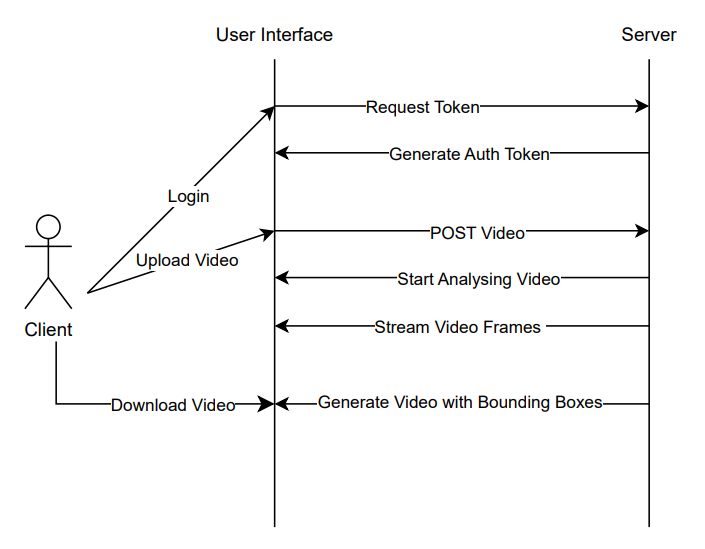
\includegraphics[width=\linewidth]{figs/flow2.png}
        \caption{Upload/Download Video Flow}
        \label{fig:flow2}
    \end{subfigure}
    \caption{Basic Client-Server Interaction Flows}
    \label{fig:flows}
\end{figure}

The \ref{fig:flow1} flow begins with the client logging into the system, establishing a secure session 
through user authentication. Following successful login, the client requests an authentication token, which the 
server generates and sends back. This token is crucial for validating the subsequent requests by the client under 
the secure session.

Once authenticated, the client requests access to the cameras associated with their account. The server responds by 
retrieving and sending a list of available cameras. The user selects a camera from this list, and the client sends a 
request to access the selected camera. The server, upon receiving this request, starts streaming video from the chosen 
camera directly to the client.

During the streaming, if the server's analysis algorithms detect a weapon in the video, it triggers an alert. 
This alert is then sent to the client, notifying them of the potential threat.

The second flow, \ref{fig:flow2}, also starts with the client logging in and obtaining an authentication token, ensuring a 
secure environment for data exchange. After login, the client uploads a video file for analysis, using a POST 
request. This video is selected from the user's local device and is sent to the server.

Upon receiving the video, the server initiates the analysis using a pre-trained object detection algorithm. 

After completing the analysis, the server generates a new version of the video, which is the output 
of the model, featuring bounding boxes around the detected objects. This annotated video is then made 
available for the client to download.

\subsection{Data Models}

In Django, models play a crucial role by serving as the structural foundation of the database. 
These models, represented in image \ref{fig:db-schema}, enable the seamless translation of database schemas into Django objects, facilitating CRUD 
(Create, Read, Update, Delete) operations through Python code, bypassing the need for direct SQL interaction.

\begin{figure}[h]
    \centering 
    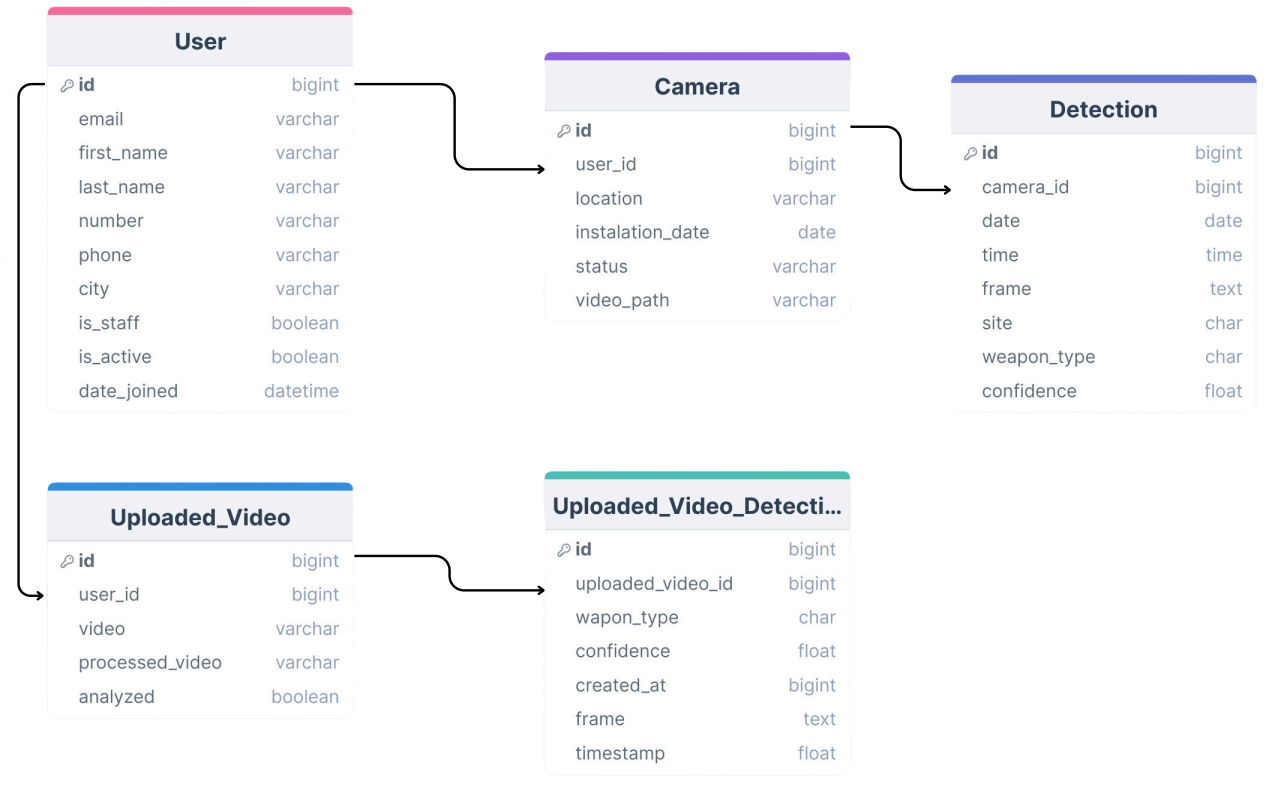
\includegraphics[width=0.8\textwidth]{figs/database-schema2.png} 
    \caption{Database Schema}
    \label{fig:db-schema}
\end{figure}

The User model at the core of this schema stores not only the credentials that officers use to access the application 
but also their personal information such as the name, contact number, and city of residence. This model also includes 
access control attributes, such as staff privileges, for managing 
permissions within the application.

Each police officer using the platform can manage multiple cameras. These cameras, detailed in the Camera model, 
are installed in various locations and are integral to capturing continuous video footage. The Detection model is 
essential for logging specific events detected by the cameras. It captures critical details such as the date, time, 
frame of detection, and the type of weapon detected, if any, along with the detection's confidence level. This 
information is vital not only for real-time alerts but also for historical data analysis, which is essential for 
post-event investigations.

Furthermore, the application supports an upload feature, allowing officers to upload video files for analysis. 
The Uploaded Video model maintains a direct association with the user, ensuring clear accountability for each 
video uploaded. It tracks whether each video has been analyzed, helping in the workflow management of video processing.

The Uploaded Video Detection model focus on detections within the uploaded videos. 
It records similar details as the Detection model, such as the type of weapon detected, the confidence level of 
the detection, and the specific frame and time within the video where the detection occurred.
\subsection{API Endpoints}
Views are a crucial component that handle the logic and control flow of applications by responding to requests from users.
Views interact with models and render appropriate responses, usually in the form of HTML pages, JSON, or XML, depending 
on the application's requirements.

The application is structured around three principal groups of endpoints, each dedicated to a specific aspect of 
the application's functionality: user management, detections, and uploaded videos. 

The first group of endpoints, \ref{fig:views-user}, focuses on user management, facilitating secure and straightforward user 
interactions with the application. The primary entry point is the login endpoint, where users authenticate by 
submitting their credentials. Successful authentication returns a session token, crucial for maintaining a 
secure and personalized session. Once authenticated, users can retrieve their profile information such as 
name, email, and role within the application.

\begin{figure}[h]
    \centering 
    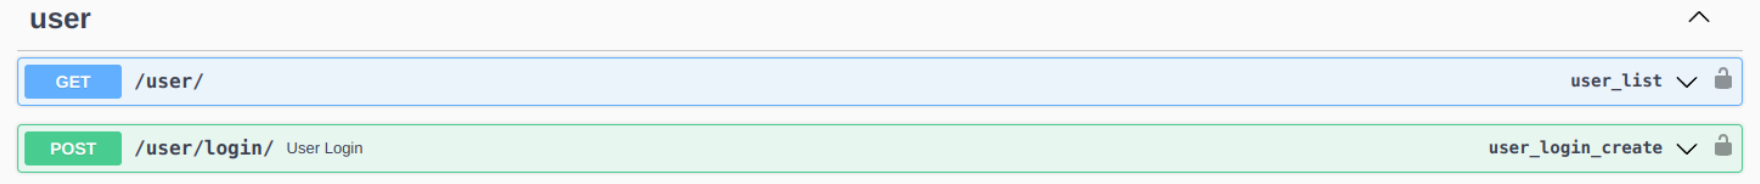
\includegraphics[width=0.95\textwidth]{figs/views-user.png} 
    \caption{User Views}
    \label{fig:views-user}
\end{figure}

Detections play a crucial role in the application, supporting both real-time security monitoring and 
historical data analysis. The POST /detections/ endpoint is designed for the application to 
submit new detection records to the database in real time when an incident is detected by a specific camera.

On the other hand, the GET method allows the application to retrieve all detection records for all cameras associated 
with a specific user. This endpoint is particularly helpful for creating a historical overview of detections,
which users can access to review and analyze past incidents.

\begin{figure}[h]
    \centering 
    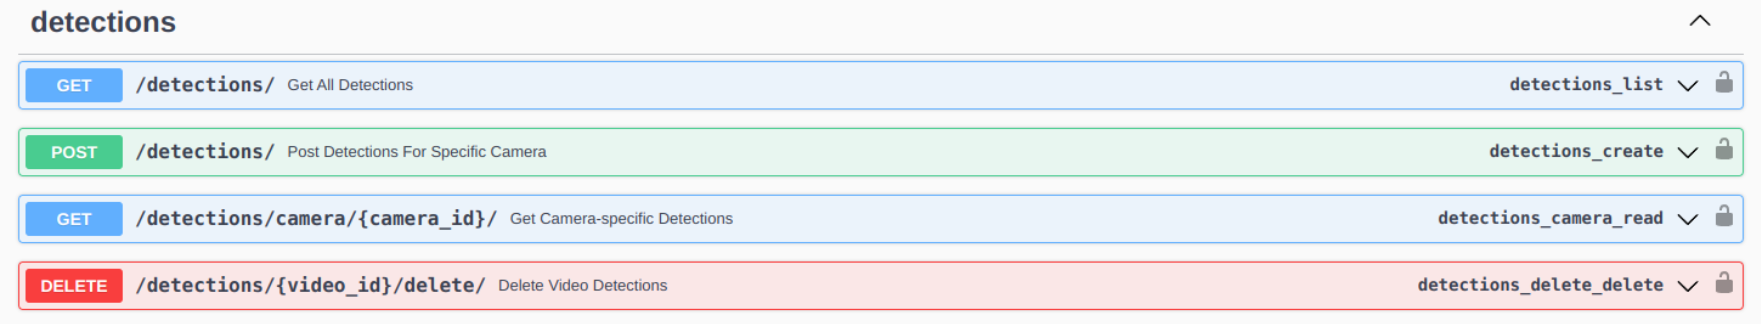
\includegraphics[width=0.95\textwidth]{figs/views-detections.png} 
    \caption{Detections Views}
    \label{fig:views-detections}
\end{figure}

Additionally, the application includes a DELETE endpoint, for the 
removal of detections associated with a particular video. This feature enables the management of stored detection data. 

The uploaded videos section of the application addresses the need to analyze previously recorded or 
externally sourced video footage. Users can upload videos through the upload video endpoint, which processes and 
stores the videos in the database, linking them to the user's account for secure and easy access.
\begin{figure}[h]
    \centering 
    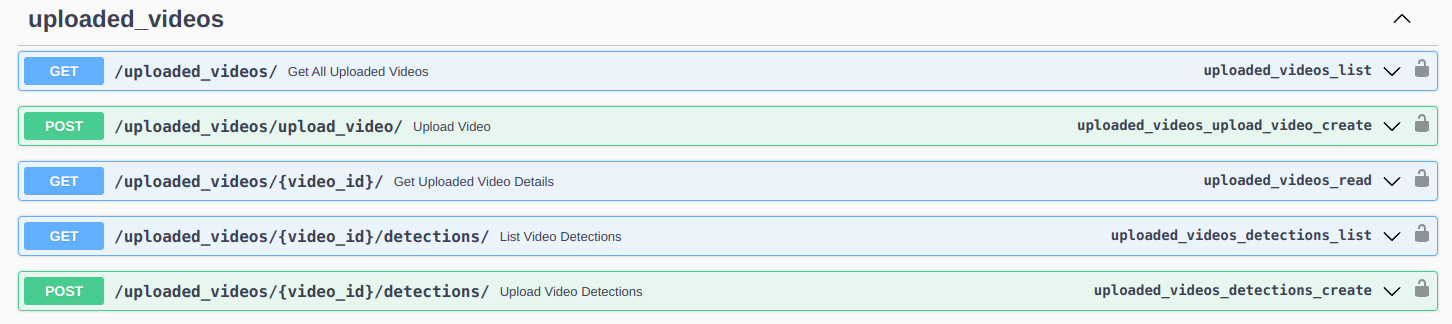
\includegraphics[width=0.95\textwidth]{figs/views-videos.png} 
    \caption{Uploaded Video Views}
    \label{fig:views-video}
\end{figure}

The application also includes a \textit{/metrics/} endpoint, which exposes Prometheus metrics using 
\textit{django\_prometheus}. This endpoint provides essential performance and operational metrics for the 
application, facilitating monitoring and alerting. These metrics cover a range of data points, such as request rates, 
response times, and error rates. This feature will be discussed in more detail in the subsequent sections.


\subsection{Django Consumers}
This section discusses the three distinct types of consumers used in the 
application: \textit{VideoStreamConsumer}, \textit{MultiCameraStreamConsumer}, and \textit{UploadedVideoStreamConsumer}.

The core of these consumers' operations begins with the initialization of the computational environment, 
specifically using \ac{gpu} acceleration via \ac{cuda} for real-time video analysis.

All consumers initiate their processing by setting up the necessary computational resources to ensure efficient 
video analysis. This setup involves determining the availability of a \ac{gpu} and utilizing 
\ac{cuda} (Compute Unified Device Architecture) for accelerated computing \ref{lbl:cuda-init}. DataParallel is used 
to distribute the model across multiple \ac{gpu}s if more than one \ac{gpu} is available.

\begin{listing}[h]
    \begin{minted}{python}
    device = "cuda" if torch.cuda.is_available() else "cpu"

    # load model and wrap it with DataParallel if multiple GPUs are available
    model = torch.hub.load('ultralytics/yolov5', 'custom', path='base/best.pt').to(device)
    if torch.cuda.device_count() > 1:
        print(f"Using {torch.cuda.device_count()} GPUs!")
        model = DataParallel(model)
    \end{minted}
    \caption{Cuda Initialization.}
    \label{lbl:cuda-init}
    \end{listing}

The \textit{VideoStreamConsumer} is fitted for handling real-time camera footage. Upon a user's selection of a camera, 
this consumer connects to RabbitMQ. 
The primary function of this consumer is to continuously receive and analyze the incoming video stream. 
It employs the initialized \ac{yolo}v5 model to detect weapons in the footage, ensuring immediate response and 
alerting in potentially threatening situations. To optimize performance, only every 10th frame of the video stream 
is analyzed, as there are not many differences between consecutive frames, making it unnecessary to analyze each one.

For scenarios where multiple camera feeds need to be monitored simultaneously, the \textit{MultiCameraStreamConsumer} 
is utilized. This consumer fetches video streams of all selected user cameras from RabbitMQ, managing multiple 
feeds efficiently. In the application interface, it lists these camera feeds, allowing users to monitor various 
viewpoints within a single dashboard.
Similar to the other consumer, also analyzes only every 10th frame of each video stream.

The \textit{UploadedVideoStreamConsumer} addresses the needs of users who upload pre-recorded videos for analysis. 
Similar to the other consumers, it streams and analyzes the uploaded video concurrently. This consumer is particularly 
important for post-event analysis.

\subsection{Database Integration}
MySQL \cite{rfc58} provides a robust, reliable, and efficient storage solution that supports the high demands of 
real-time data processing and retrieval.

The integration of MySQL within the application infrastructure is facilitated through its deployment inside a 
Docker container. This approach simplifies the process of setting up and managing the database 
environment. Encapsulating the MySQL instance in a Docker container, ensures a consistent environment 
across all stages of development and production, which helps in reducing potential discrepancies that 
can arise from environment-specific configurations.

To connect the Django application to the MySQL database, the necessary configurations are in the \textit{settings.py} 
file of the Django project.

%or this detection system, the data involves structured information such as timestamps, locations, frame details, 
%and metadata from surveillance footage, which are inherently relational and fit well into the tabular format of 
%SQL databases.

In the context of this detection system, data primarily consists of structured information such as timestamps, 
locations, frame details, and metadata extracted from surveillance footage. Given the relational nature of this data, 
it aligns well with the tabular format inherent to SQL databases. Utilizing MySQL enables efficient storage, querying, 
and manipulation of this data, thereby enhancing the overall performance of the detection system.

\subsection{\ac{yolo} Model Integration}
The integration of the pretrained \ac{yolo} model into the backend for video analysis involved several key steps:

\begin{itemize}
    \item Model Pre-training: the \ac{yolo} model is first pretrained on the custom dataset to detect objects, 
    as detailed in the section below;
    \item Environment Setup: the necessary packages and dependencies are installed;
    \item Model Integration: pretrained \ac{yolo} model's weight file was incorporated into the Django app;
    \item Video Processing: within the Django app, views are set up to handle video processing. When a camera is 
    selected, the video feed is processed in real-time using the \ac{yolo} model to detect weapons.
\end{itemize}

\section{Web Server Configuration}
\subsection{Nginx Setup and Load Balancing}
Load balancing is crucial for maintaining 
optimal performance, especially under high traffic conditions, as it ensures consistent response times and maximizes 
resource utilization.
Nginx \cite{rfc57} functions as a high-performance web server and reverse proxy server within the system, efficiently managing 
incoming HTTP and WebSocket requests. It enhances the system's reliability and scalability by distributing client 
requests to various backend services. This setup ensures load balancing and efficient resource utilization.

Nginx is deployed using docker-compose with the \textit{nginx:latest} image, ensuring that Nginx uses the specified 
configuration file (nginx.conf).

Load balancing consists of distributing network or application traffic across multiple servers to ensure no single 
server becomes overwhelmed. This technique enhances the availability and reliability of applications by preventing 
server overloads and ensuring that client requests are efficiently managed.

Nginx employs load balancing through defined upstream server pools. The \textit{upstream} directive specifies a group of 
backend servers to distribute requests. Two upstream pools are configured: \textit{backend\_api} for API requests 
and \textit{backend\_ws} for websocket connections, as shown in listing \ref{lbl:nginx-setup}.


\begin{listing}[h]
    \begin{minted}{nginx}
    # Define upstream server pool for API
    upstream backend_api {
        least_conn;
        server 172.17.0.1:8000;
        server 172.17.0.1:8001;
        server 172.17.0.1:8002; 
    }

    # Define upstream server pool for WebSocket connections
    upstream backend_ws {
        server 172.17.0.1:8000;
        server 172.17.0.1:8001;
        server 172.17.0.1:8002;
    }
    \end{minted}
    \caption{Nginx Configuration Setup}
    \label{lbl:nginx-setup}
    \end{listing}

For \textit{backend\_api}, Nginx uses the least\_conn load balancing method. This method directs incoming requests to the 
server with the fewest active connections, ensuring an even load distribution across all servers in the pool.

The configuration for WebSocket connections under \textit{backend\_ws} also distributes requests among the same set of
backend servers, maintaining efficient handling of persistent connections.

Nginx listens on port 8080 and routes requests based on URL paths.
For the root location, requests to \textit{/} are proxied to a frontend service on port 3000, including 
headers to forward client details. Requests to \textit{/api/} are forwarded to the backend API servers with headers 
to maintain client information and a 100MB limit for uploads.
For websocket connections, requests to \textit{/ws/} are directed to the backend WebSocket servers with the necessary 
headers for WebSocket connections.

%\begin{figure}[h]
%    \centering 
%    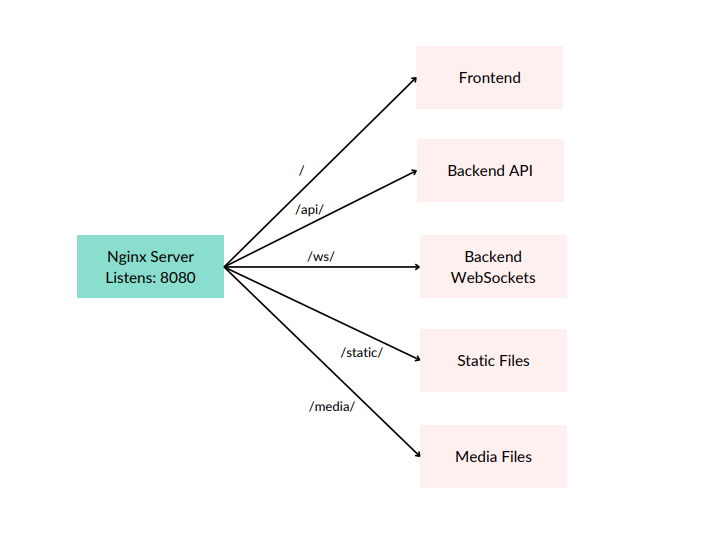
\includegraphics[width=0.6\textwidth]{figs/nginx-conf.png} 
%    \caption{Nginx Load Balancing}
%    \label{fig:nginx-conf}
%\end{figure}

\section{Monitoring and Visualization}
\subsection{Metrics Collection with Prometheus}
Prometheus \cite{rfc56} is an open-source systems monitoring and alerting toolkit designed primarily for reliability and scalability.
It works by scraping metrics from applications, storing this data in a time-series database, and allowing 
powerful queries and visualizations through its flexible query language.

It collects metrics data through a "scraping" process. This involves periodically querying an endpoint on 
the application that exposes metrics, \textit{/metrics/}. The application has been instrumented with 
django\_prometheus to provide these metrics.

Prometheus is launched using Docker and configured via a YAML file \textit{prometheus.yml}, exposing Prometheus 
on port 9090.


\subsection{Visualization using Grafana}
Grafana \cite{rfc55} is an open-source analytics and interactive visualization web application. It is highly extensible and 
provides tools to build dashboards for visualizing data from various sources, including Prometheus. Grafana supports 
a wide range of chart types and is used to create real-time, dynamic dashboards that help monitor and analyze system 
performance.

Grafana is crucial for interpreting the raw data collected by Prometheus. It connects to Prometheus, queries its 
time-series database, and presents the data in an accessible, visual format.

Grafana was deployed using Docker and configured to run on port 3001, depending on Prometheus being available 
to function correctly.

A dashboard was created featuring several metrics, as represented in figure \ref{fig:grafana-dashboard}. This allows for 
a comprehensive understanding of the application's behavior, facilitating detailed performance analysis and issue 
detection.

\begin{figure}[h]
    \centering 
    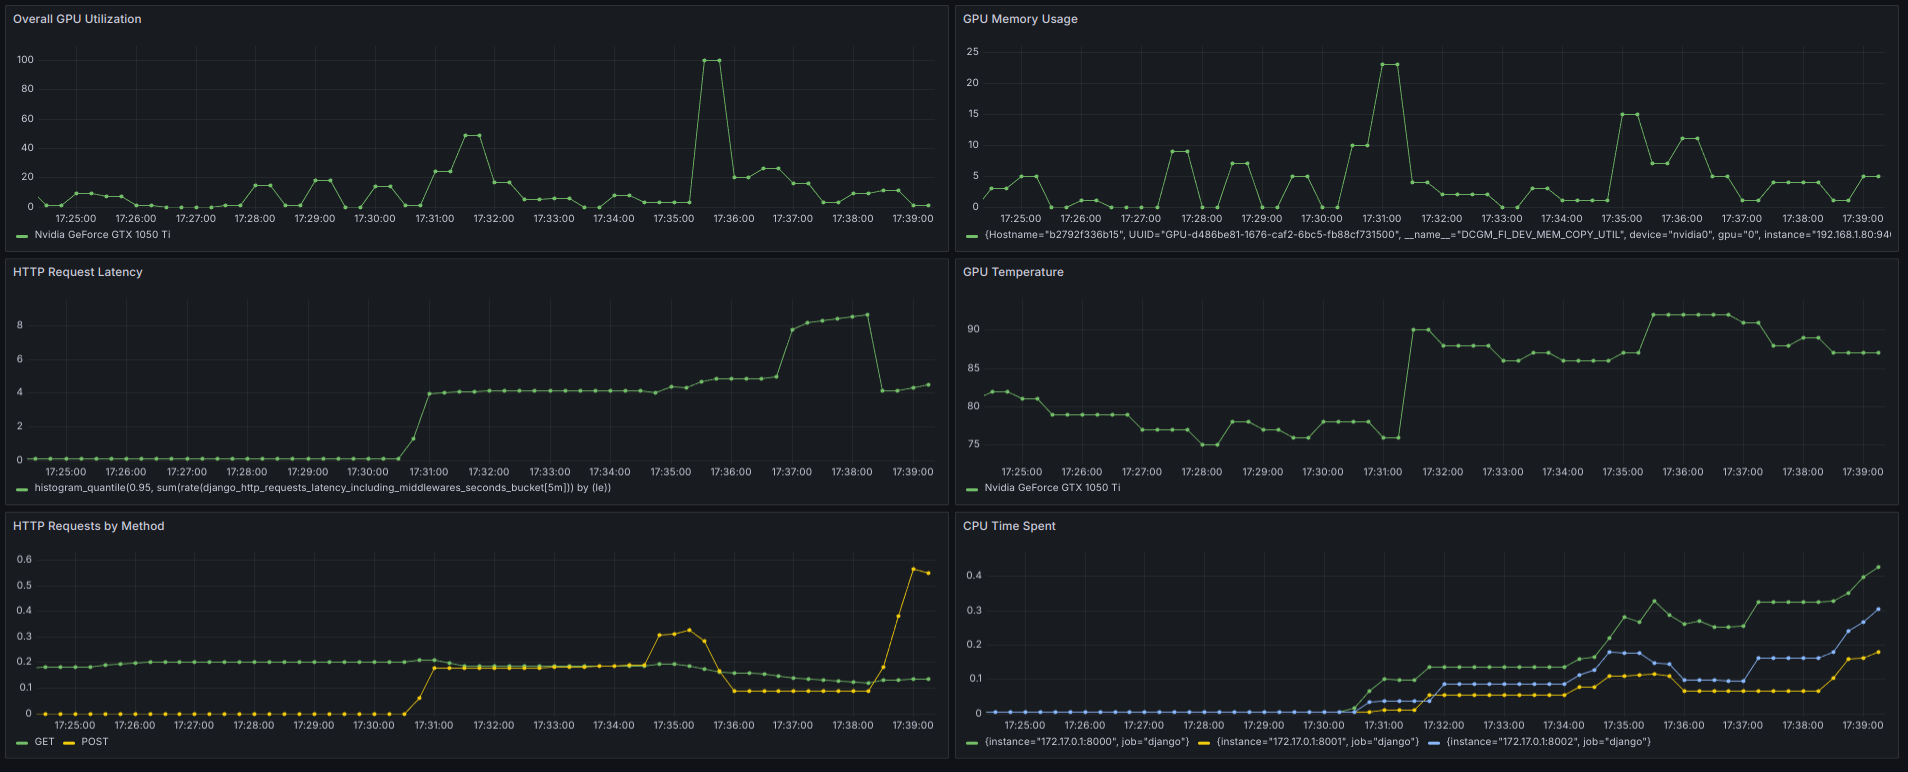
\includegraphics[width=0.98\textwidth]{figs/grafana-dashboard.png} 
    \caption{Grafana Dashboard}
    \label{fig:grafana-dashboard}
\end{figure}

\section{Implementation Challenges}
Implementing real-time weapon analysis for surveillance systems presents a series of significant challenges, 
primarily centered on balancing the trade-offs between speed, resolution, and system resources.

One of the difficulties arises from the key requirement to analyze and stream video content with minimal delay. 
Real-time processing is essential for effective surveillance, allowing for immediate response to potential security 
incidents as they occur. However, achieving this level of promptness often necessitates compromises in other aspects 
of the system.

A critical compromise involves the resolution of the video footage. To facilitate faster processing and streaming, 
it is often necessary to reduce the resolution of the video. This reduction speeds up the analysis by reducing the 
data load on the system, thus minimizing the delay in video streaming. However, lower resolution images can significantly 
degrade the quality of the surveillance footage.

Furthermore, the scalability of real-time video analysis systems is another major challenge, particularly when multiple 
cameras are integrated into the surveillance network. As the number of cameras increases, so too does the overload on the 
system's computational resources, including CPU and \ac{gpu} capacities. This escalation can lead to slower processing times 
and increased delays in video analysis and streaming, thereby compromising the real-time capability of the system.
%\subsection{Synchronization Issues}
\section{Scalability and Performance Optimizations}
To ensure the system can handle increasing workloads and deliver optimal performance, several 
scalability and performance optimizations were implemented across all components.

In the frontend, Web Workers were utilized to handle frame processing in the background, offloading intensive 
tasks from the main thread and keeping the user interface responsive and fluid.
Additionally, the number of DOM updates in canvas components was reduced by batching multiple updates and limiting 
unnecessary interactions with the DOM. This approach achieved smoother rendering and improved visual performance.
By managing state effectively, unnecessary calls to external services were minimized. For example, instead of making 
multiple calls to RabbitMQ, a single persistent connection was established.

On the backend, a dedicated worker pool was employed to handle frame processing in parallel. This setup took 
advantage of multi-core processors, distributing the workload among multiple workers and significantly increasing 
the system's throughput and scalability. Unused memory was periodically cleared to prevent memory leaks and maintain 
efficient memory usage.
The frequency of frames analyzed by the object detection algorithm was reduced, processing every 10th frame 
instead of every frame to balance performance with accuracy and reduce computational demands without significantly 
compromising detection capabilities.
Batch processing for frames was also implemented, allowing multiple frames to be processed simultaneously rather 
than individually, thus maximizing the \ac{gpu}'s parallel processing power.

For RabbitMQ various settings were optimized to achieve better performance. The prefetch count was increased to 
allow RabbitMQ to send more messages to consumers without waiting for acknowledgments, reducing latency and improving 
throughput.


%%%%%%%%%%%%%%%%%%%%%%%%%%%%%%%%%%%%%%%%%%%%%%%%%%%%%%%
% End of Thesis text 
%%%%%%%%%%%%%%%%%%%%%%%%%%%%%%%%%%%%%%%%%%%%%%%%%%%%%%%

\backmatter

%%%%%%%%%%%%%%%%%%%%%%%%%%%%%%%%%%%%%%%%%%%%%%%%%%%%%%%
% Print all used references
%%%%%%%%%%%%%%%%%%%%%%%%%%%%%%%%%%%%%%%%%%%%%%%%%%%%%%%

\begingroup
\renewcommand{\bibfont}{\footnotesize}
% Redefine References name to Portuguese
% Change if you are using english
\defbibheading{bibliography}[Referências]{
	\chapter{#1}
}
\SingleSpacing
\setlength\bibitemsep{8pt}
\printbibliography[heading=bibliography]
\endgroup


%%%%%%%%%%%%%%%%%%%%%%%%%%%%%%%%%%%%%%%%%%%%%%%%%%%%%%%
% Load appendix
%%%%%%%%%%%%%%%%%%%%%%%%%%%%%%%%%%%%%%%%%%%%%%%%%%%%%%%

\mainmatterWithoutReset
\appendix

% \include{appendix-a}
% \include{appendix-b}
% \include{appendix-c}

\end{document}
